\documentclass[11pt]{article}

%
%
%
\usepackage[margin=0.78in]{geometry}
\usepackage{amsmath,amssymb,amsfonts,mathtools}
\usepackage{booktabs,array,tabularx,longtable,multirow}
\usepackage{enumitem}
\usepackage[most]{tcolorbox}
\usepackage{xcolor}
\usepackage{fancyhdr}
\usepackage{titlesec}
\usepackage{hyperref}
\usepackage{lastpage}
\usepackage{setspace}
\usepackage{tikz}
\usepackage{pgfplots}
\usepackage{needspace}
\usepackage{caption}
\usepackage{multicol}
\usepackage{graphicx}
\usepackage{amsthm}
\usepackage{mathrsfs}
\usepackage{bm}
\usepackage{float}
\usepackage{colortbl}
\usepackage{tocloft}

\pgfplotsset{compat=1.18}
\setstretch{1.16}
\setlength{\parindent}{0pt}
\setlength{\parskip}{0.45em}
\setlist[itemize]{leftmargin=1.8em}
\setlist[enumerate]{leftmargin=2em}

%
%
%
\definecolor{novelPurple}{RGB}{106,76,230}
\definecolor{novelPurpleDark}{RGB}{76,50,180}
\definecolor{novelPurpleLight}{RGB}{244,241,255}
\definecolor{novelPurpleLine}{RGB}{188,170,255}
\definecolor{npgray}{RGB}{78,78,78}
\definecolor{softgray}{RGB}{246,246,250}
\definecolor{softlav}{RGB}{250,248,255}
\definecolor{greencheck}{RGB}{24,128,88}
\definecolor{warmred}{RGB}{188,54,54}

%
%
%
\hypersetup{
    colorlinks=true,
    linkcolor=novelPurpleDark,
    urlcolor=novelPurpleDark,
    citecolor=novelPurpleDark
}

%
%
%
\pagestyle{fancy}
\setlength{\headheight}{14pt}
\fancyhf{}
\fancyhead[L]{\textbf{Novel Prep Learning Center}}
\fancyhead[R]{\textbf{AP Calculus AB --- Unit 1}}
\fancyfoot[C]{\textcolor{novelPurpleDark}{\thepage\ /\ \pageref{LastPage}}}
\renewcommand{\headrulewidth}{0.4pt}
\renewcommand{\footrulewidth}{0pt}

%
%
%
\setcounter{secnumdepth}{2}
\setcounter{tocdepth}{1}
\renewcommand{\thesection}{1.\arabic{section}}
\renewcommand{\thesubsection}{1.\arabic{section}.\arabic{subsection}}
\renewcommand{\contentsname}{Contents}
\renewcommand{\cfttoctitlefont}{\Huge\bfseries\color{novelPurpleDark}}
\renewcommand{\cftaftertoctitle}{\hfill}
\renewcommand{\cftsecleader}{\cftdotfill{\cftdotsep}}
\renewcommand{\cftsubsecleader}{\cftdotfill{\cftdotsep}}
\setlength{\cftbeforesecskip}{7pt}
\setlength{\cftbeforesubsecskip}{2pt}
\setlength{\cftsecnumwidth}{3.2em}
\setlength{\cftsubsecnumwidth}{4.3em}
\renewcommand{\cftsecfont}{\color{novelPurpleDark}\bfseries}
\renewcommand{\cftsubsecfont}{\color{npgray}}
\renewcommand{\cftsecpagefont}{\color{novelPurpleDark}\bfseries}
\renewcommand{\cftsubsecpagefont}{\color{npgray}}

%
%
%
\titleformat{\section}
{\Large\bfseries\color{novelPurpleDark}}{\thesection.}{0.6em}{}

\titleformat{\subsection}
{\large\bfseries\color{novelPurple}}{\thesubsection.}{0.6em}{}

\titleformat{\subsubsection}
{\normalsize\bfseries\color{novelPurpleDark}}{}{0em}{}

%
%
%
\tcbset{
  enhanced,
  sharp corners,
  boxrule=0.95pt
}

%
\newtcolorbox{theorybox}[1]{
  colback=white,
  colframe=novelPurple,
  colbacktitle=novelPurple,
  coltitle=white,
  title={\large\textbf{#1}},
  fonttitle=\bfseries,
  sharp corners,
  enhanced,
  breakable,
  boxrule=0.95pt
}

%
\newtcolorbox{notebox}[1]{
  colback=softlav,
  colframe=novelPurple,
  colbacktitle=novelPurple,
  coltitle=white,
  title={\large\textbf{#1}},
  fonttitle=\bfseries,
  sharp corners,
  enhanced,
  breakable,
  boxrule=0.95pt
}

%
\newtcolorbox{skillbox}[1]{
  colback=novelPurpleLight,
  colframe=novelPurpleDark,
  colbacktitle=novelPurpleDark,
  coltitle=white,
  title={\large\textbf{#1}},
  fonttitle=\bfseries,
  sharp corners,
  enhanced,
  breakable,
  boxrule=0.95pt
}

%
\newtcolorbox{bigideabox}[1]{
  colback=white,
  colframe=novelPurple,
  colbacktitle=novelPurple,
  coltitle=white,
  title={\large\textbf{#1}},
  fonttitle=\bfseries,
  sharp corners,
  enhanced,
  breakable,
  boxrule=1pt
}

\newcommand{\ds}{\displaystyle}
\newcommand{\R}{\mathbb{R}}

%
%
%
\newcounter{examplectr}[section]
\renewcommand{\theexamplectr}{\thesection.\arabic{examplectr}}

\newcommand{\example}[1]{%
\refstepcounter{examplectr}
\noindent{\color{novelPurpleDark}\textbf{Example \theexamplectr.}} \textbf{#1}
}

\newcommand{\solution}{\noindent{\textbf{Solution.}}}

\newcommand{\apcheckpoint}[1]{%
\begin{skillbox}{AP Checkpoint}
#1
\end{skillbox}
}

\begin{document}

%
%
%
\begin{titlepage}
\centering
\vspace*{2.0cm}

{\fontsize{28}{32}\selectfont\bfseries\color{novelPurpleDark} AP Calculus AB\par}
\vspace{0.4cm}
{\fontsize{28}{32}\selectfont\bfseries\color{novelPurpleDark} Unit 1: Limits and Continuity\par}
\vspace{0.15cm}
{\Large\color{npgray} Limits and Continuity Foundations\par}


\vspace{1.0cm}

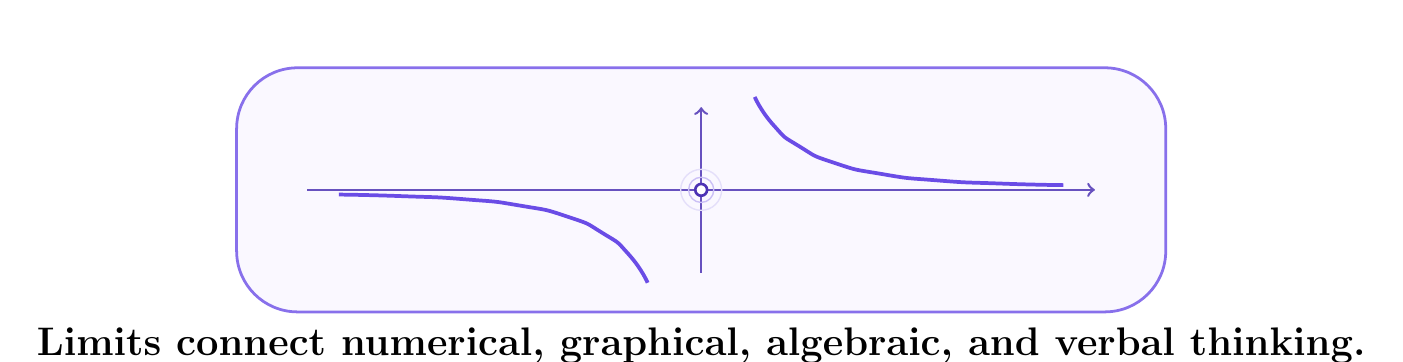
\begin{tikzpicture}[scale=1]

%
\fill[softlav, rounded corners=22pt] (-5.9,-1.55) rectangle (5.9,1.55);
\draw[novelPurple!80, line width=1pt, rounded corners=22pt] (-5.9,-1.55) rectangle (5.9,1.55);

%
\draw[novelPurpleDark!85, line width=0.9pt, ->] (-5.0,0) -- (5.0,0);

%
\draw[novelPurpleDark!85, line width=0.9pt, ->] (0,-1.05) -- (0,1.05);

%
\draw[novelPurple, line width=1.35pt, smooth]
  plot [tension=1.05] coordinates {
    (-4.6,-0.06) (-3.8,-0.08) (-3.0,-0.12) (-2.3,-0.20)
    (-1.7,-0.34) (-1.25,-0.55) (-0.92,-0.82) (-0.68,-1.18)
  };

%
\draw[novelPurple, line width=1.35pt, smooth]
  plot [tension=1.05] coordinates {
    (0.68,1.18) (0.92,0.82) (1.25,0.55) (1.7,0.34)
    (2.3,0.20) (3.0,0.12) (3.8,0.08) (4.6,0.06)
  };

%
\fill[white] (0,0) circle (0.075);
\draw[novelPurpleDark, line width=0.95pt] (0,0) circle (0.075);

%
\draw[novelPurple!35, line width=0.5pt] (0,0) circle (0.16);
\draw[novelPurple!18, line width=0.5pt] (0,0) circle (0.26);

%
\node[align=center, text=black] at (0,-1.98)
{\Large\bfseries Limits connect numerical, graphical, algebraic, and verbal thinking.};

\end{tikzpicture}
\vfill

\begin{minipage}{0.83\textwidth}
\begin{notebox}{What You Will Learn}
\begin{itemize}
    \item Interpret limits from graphs, tables, formulas, and verbal descriptions.
    \item Choose efficient methods for indeterminate forms and one-sided behavior.
    \item Explain continuity, classify discontinuities, and repair removable holes.
    \item Analyze vertical and horizontal asymptotes with correct limit notation.
    \item Use the Intermediate Value Theorem to prove that a value must occur.
\end{itemize}
\end{notebox}
\end{minipage}

\vfill

{\large\textbf{Novel Prep Learning Center}}\\[0.25em]

\end{titlepage}

\clearpage
\thispagestyle{fancy}
\tableofcontents
\newpage

%
%
%
\section*{Unit Overview}
\addcontentsline{toc}{section}{Unit Overview}

\begin{skillbox}{Unit 1 Structure}
This unit builds limits and continuity as one connected story. The chapter is organized around the following ideas:
\begin{enumerate}
    \item introducing change and instantaneous behavior
    \item defining limits and reading notation correctly
    \item estimating limits from graphs and tables
    \item evaluating limits with algebraic properties and algebraic manipulation
    \item selecting appropriate strategies, including the Squeeze Theorem
    \item connecting multiple representations of limits
    \item classifying discontinuities and studying continuity
    \item understanding infinite limits, asymptotes, and the Intermediate Value Theorem
\end{enumerate}
\end{skillbox}

\begin{theorybox}{AP Unit 1 Topic Map}
\renewcommand{\arraystretch}{1.28}
\begin{tabularx}{\textwidth}{>{\bfseries}p{0.16\textwidth} X >{\raggedright\arraybackslash}p{0.28\textwidth}}
\toprule
Topic & Focus & Main Skill Emphasis \\
\midrule
1.1 & Introducing Calculus: Can Change Occur at an Instant? & interpret changing behavior conceptually \\
1.2 & Defining Limits and Using Limit Notation & read and communicate limit notation \\
1.3 & Estimating Limit Values from Graphs & graphical interpretation \\
1.4 & Estimating Limit Values from Tables & numerical interpretation \\
1.5 & Determining Limits Using Algebraic Properties & direct substitution and limit laws \\
1.6 & Determining Limits Using Algebraic Manipulation & factoring, rationalizing, common denominators \\
1.7 & Selecting Procedures for Determining Limits & choosing the best method \\
1.8 & Determining Limits Using the Squeeze Theorem & bounding arguments \\
1.9 & Connecting Multiple Representations of Limits & translation between forms \\
1.10 & Exploring Types of Discontinuities & classify non-continuity \\
1.11 & Defining Continuity at a Point & apply the 3-condition definition \\
1.12 & Confirming Continuity over an Interval & continuity on intervals and endpoints \\
1.13 & Removing Discontinuities & removable holes and redefining functions \\
1.14 & Infinite Limits and Vertical Asymptotes & behavior near excluded points \\
1.15 & Limits at Infinity and Horizontal Asymptotes & end behavior \\
1.16 & Intermediate Value Theorem & existence arguments and AP justification \\
\bottomrule
\end{tabularx}
\end{theorybox}

\begin{notebox}{Teaching Philosophy for This Unit}
Students should not learn limits as a list of tricks. They should see limits as the language that describes \emph{approach behavior}. In this unit, every major idea appears in multiple forms: graph, table, algebra, and words. That is the key to lasting understanding.
\end{notebox}

\newpage
\setcounter{section}{0}

%
%
%
\section{Introducing Calculus: Can Change Occur at an Instant?}

\begin{bigideabox}{Big Idea}
One of the central questions of calculus is this:

\begin{center}
\emph{How can we describe what is happening at an instant when change usually takes time?}
\end{center}

Average rate of change looks over an interval. Instantaneous change asks what happens at a single moment. Limits are the tool that make this possible.
\end{bigideabox}

Suppose a particle travels along a line and its position is
\[
s(t)=t^2+1.
\]
Over the interval from $t=2$ to $t=3$, the average rate of change is
\[
\frac{s(3)-s(2)}{3-2}=\frac{10-5}{1}=5.
\]
But what if we want the rate of change \emph{at} $t=2$ exactly? That leads to expressions such as
\[
\frac{s(2+h)-s(2)}{h}
\]
and then to the limit as $h\to 0$.

\example{Motivating instantaneous change with a secant slope.}

For
\[
s(t)=t^2+1,
\]
compute the average rate of change from $t=2$ to $t=2+h$, and simplify.

\bigskip

\solution

\[
\frac{s(2+h)-s(2)}{h}
=
\frac{(2+h)^2+1-(2^2+1)}{h}
\]
\[
=
\frac{4+4h+h^2+1-5}{h}
=
\frac{4h+h^2}{h}
=
4+h.
\]

So as $h\to 0$, the average rate of change approaches
\[
4.
\]

\bigskip

\apcheckpoint{Why is the expression $4+h$ more useful than the original fraction? Because after simplification, we can see what value the rate is approaching as the interval length shrinks.}

\newpage

%
%
%
\section{Defining Limits and Using Limit Notation}

\subsection{What a Limit Means}

\begin{theorybox}{Definition of a Limit (Informal)}
When we write
\[
\lim_{x\to c}f(x)=L,
\]
we mean that as $x$ gets arbitrarily close to $c$, the value of $f(x)$ gets arbitrarily close to $L$.
\end{theorybox}

\begin{theorybox}{Important Clarification}
A limit describes what the function is \emph{approaching}, not necessarily what the function \emph{equals} at the point.
\end{theorybox}

\begin{theorybox}{Formal Definition (Optional Precision)}
Let $f$ be defined on an open interval containing $c$, except possibly at $c$ itself. We say
\[
\lim_{x\to c}f(x)=L
\]
if for every $\varepsilon>0$, there exists a $\delta>0$ such that whenever
\[
0<|x-c|<\delta,
\]
it follows that
\[
|f(x)-L|<\varepsilon.
\]
\end{theorybox}

\subsection{Reading the Notation}

\[
\lim_{x\to 3}f(x)=5
\]
is read as:

\begin{center}
\emph{``The limit of $f(x)$ as $x$ approaches $3$ is $5$.''}
\end{center}

This does \emph{not} automatically mean that $f(3)=5$.

\example{Separating the function value from the limit value.}

Suppose
\[
f(x)=
\begin{cases}
x+2, & x\neq 3,\\[0.2em]
10, & x=3.
\end{cases}
\]
Find $\lim_{x\to 3}f(x)$ and compare it to $f(3)$.

\bigskip

\solution

For all $x\neq 3$, the function behaves like $x+2$. Therefore,
\[
\lim_{x\to 3}f(x)=\lim_{x\to 3}(x+2)=5.
\]
But by definition,
\[
f(3)=10.
\]

So
\[
\lim_{x\to 3}f(x)=5
\qquad\text{while}\qquad
f(3)=10.
\]

These are different.

\bigskip

\begin{notebox}{Key Message}
A function can have a limit at $x=c$ even if:
\begin{itemize}
    \item the function is not defined at $x=c$, or
    \item the function value at $x=c$ does not equal the limit.
\end{itemize}
\end{notebox}

\newpage

%
%
%
\section{Estimating Limit Values from Graphs}

\begin{theorybox}{Graphical Strategy}
To estimate
\[
\lim_{x\to c}f(x),
\]
look at the $y$-values the graph approaches from the left and from the right as $x$ gets close to $c$.
\end{theorybox}

\subsection{A Visual Example}

\begin{center}
\begin{tikzpicture}[scale=1.08]
\begin{axis}[
    axis lines=middle,
    xmin=-1.2,xmax=4.6,
    ymin=-0.8,ymax=4.8,
    width=12.2cm,
    height=7.0cm,
    xtick={0,1,2,3,4},
    ytick={0,1,2,3,4},
    xlabel={$x$},
    ylabel={$y$},
    every axis x label/.style={at={(current axis.right of origin)}, anchor=west},
    every axis y label/.style={at={(current axis.above origin)}, anchor=south},
    clip=false
]
\addplot[novelPurpleDark, very thick, domain=-1:2, samples=200] {x+1};
\addplot[novelPurpleDark, very thick, domain=2:4.4, samples=200] {-x+5};
\addplot[novelPurpleDark, only marks, mark=*, mark size=2.2pt] coordinates {(2,1.5)};
\addplot[novelPurpleDark, only marks, mark=o, mark size=2.4pt] coordinates {(2,3)};
\end{axis}
\end{tikzpicture}
\end{center}

From the graph:
\[
\lim_{x\to 2^-}f(x)=3,
\qquad
\lim_{x\to 2^+}f(x)=3.
\]
Therefore,
\[
\lim_{x\to 2}f(x)=3.
\]
But the solid point is at
\[
f(2)=1.5.
\]

\example{Reading a limit from a graph.}

Use the graph above to determine:
\[
\lim_{x\to 2}f(x),\qquad f(2),\qquad \text{and whether }f\text{ is continuous at }x=2.
\]

\bigskip

\solution

From both sides, the graph approaches $3$, so
\[
\lim_{x\to 2}f(x)=3.
\]
The solid point gives the actual function value:
\[
f(2)=1.5.
\]
Since
\[
\lim_{x\to 2}f(x)\neq f(2),
\]
the function is \textbf{not continuous} at $x=2$.

\bigskip

\begin{notebox}{Graph Checklist}
When reading from a graph, always ask:
\begin{enumerate}
    \item What does the graph approach from the left?
    \item What does the graph approach from the right?
    \item Are those two values equal?
    \item Is the actual point filled in somewhere else?
\end{enumerate}
\end{notebox}

\newpage

%
%
%
\section{Estimating Limit Values from Tables}

\begin{theorybox}{Numerical Strategy}
To estimate a limit numerically, evaluate the function at inputs close to the target value from both sides and look for the output values the function approaches.
\end{theorybox}

\example{Estimating a limit numerically.}

Estimate
\[
\lim_{x\to 0}\frac{x}{\sqrt{x+1}-1}.
\]

\bigskip

\solution

We first build a table of values near $x=0$.

\begin{center}
\renewcommand{\arraystretch}{1.2}
\begin{tabular}{c|ccccccc}
\toprule
$x$ & $-0.01$ & $-0.001$ & $-0.0001$ & $0$ & $0.0001$ & $0.001$ & $0.01$ \\
\midrule
$\ds \frac{x}{\sqrt{x+1}-1}$ & $1.99499$ & $1.99950$ & $1.99995$ & undefined & $2.00005$ & $2.00050$ & $2.00499$ \\
\bottomrule
\end{tabular}
\end{center}

The output values approach $2$ from both sides, so the limit appears to be
\[
\boxed{2}.
\]

\bigskip

\begin{notebox}{Important Warning}
A table provides evidence, not a proof. A numerical estimate can suggest a limit, but later in the unit we confirm limits algebraically when possible.
\end{notebox}

\example{A table where the limit does not exist.}

Suppose a table near $x=0$ for a function $g$ gives:

\begin{center}
\renewcommand{\arraystretch}{1.2}
\begin{tabular}{c|ccc|ccc}
\toprule
$x$ & $-0.1$ & $-0.01$ & $-0.001$ & $0.001$ & $0.01$ & $0.1$ \\
\midrule
$g(x)$ & $-1.01$ & $-1.00$ & $-1.00$ & $0.99$ & $1.00$ & $1.01$ \\
\bottomrule
\end{tabular}
\end{center}

What can you conclude about $\lim_{x\to 0}g(x)$?

\bigskip

\solution

From the left side, the values approach $-1$.
From the right side, the values approach $1$.

Since the left-hand and right-hand limits are different,
\[
\lim_{x\to 0}g(x)
\]
does not exist.

\newpage

%
%
%
\section{Determining Limits Using Algebraic Properties}

\begin{theorybox}{Some Basic Limits}
For real numbers $b,c$ and positive integer $n$:
\[
\lim_{x\to c} b=b,
\qquad
\lim_{x\to c} x=c,
\qquad
\lim_{x\to c} x^n=c^n.
\]
\end{theorybox}

\begin{theorybox}{Properties of Limits}
If
\[
\lim_{x\to c}f(x)=L
\qquad\text{and}\qquad
\lim_{x\to c}g(x)=K,
\]
then:
\begin{enumerate}
    \item $\lim\limits_{x\to c}[f(x)+g(x)]=L+K$
    \item $\lim\limits_{x\to c}[f(x)-g(x)]=L-K$
    \item $\lim\limits_{x\to c}[f(x)g(x)]=LK$
    \item $\lim\limits_{x\to c}\dfrac{f(x)}{g(x)}=\dfrac{L}{K}$ if $K\neq 0$
    \item $\lim\limits_{x\to c}[f(x)]^n=L^n$
\end{enumerate}
\end{theorybox}

\begin{theorybox}{Direct Substitution Principle}
If a function is continuous at $x=c$, then
\[
\lim_{x\to c}f(x)=f(c).
\]
This works for:
\begin{itemize}
    \item polynomials
    \item rational functions where the denominator is not zero
    \item radicals when the input stays in the domain
    \item many standard elementary functions
\end{itemize}
\end{theorybox}

\example{Evaluating basic limits by substitution.}

Find:
\[
\lim_{x\to 2}(4x^2+3).
\]

\bigskip

\solution

Since polynomials are continuous everywhere, substitute directly:
\[
\lim_{x\to 2}(4x^2+3)=4(2)^2+3=16+3=19.
\]

\[
\boxed{19}
\]

\bigskip

\example{A rational function with direct substitution.}

Find:
\[
\lim_{x\to 1}\frac{x^2+x+2}{x+1}.
\]

\bigskip

\solution

Because the denominator at $x=1$ is
\[
1+1=2\neq 0,
\]
the function is continuous at $x=1$. Substitute directly:
\[
\lim_{x\to 1}\frac{x^2+x+2}{x+1}
=
\frac{1^2+1+2}{1+1}
=
\frac{4}{2}=2.
\]

\[
\boxed{2}
\]

\bigskip

\example{A composite function.}

Find:
\[
\lim_{x\to 0}\sqrt{x^2+4}.
\]

\bigskip

\solution

First evaluate the inside:
\[
x^2+4\to 0^2+4=4.
\]
Then apply the outer function:
\[
\sqrt{x^2+4}\to \sqrt{4}=2.
\]

So
\[
\boxed{2}.
\]

\bigskip
\newpage
\begin{notebox}{Procedure Selection}
Before doing complicated algebra, first ask:
\begin{center}
\emph{Can I substitute directly?}
\end{center}
If yes, that is usually the fastest correct method.
\end{notebox}

%
%
%
%
\newpage
\subsection*{1.5 Full Lesson --- Why Limit Properties Work}

\begin{bigideabox}{The Central Idea}
Suppose $f(x)$ can be made as close as we want to $L$ by taking $x$ sufficiently close to $c$, and $g(x)$ can be made as close as we want to $K$. Then ordinary arithmetic performed on the nearby outputs behaves like the same arithmetic performed on $L$ and $K$.

This is why we may split a complicated expression into simpler pieces, find the limit of each piece, and then recombine the results. The properties are not shortcuts to memorize blindly; they describe how stable arithmetic operations interact with approaching values.
\end{bigideabox}

\begin{center}
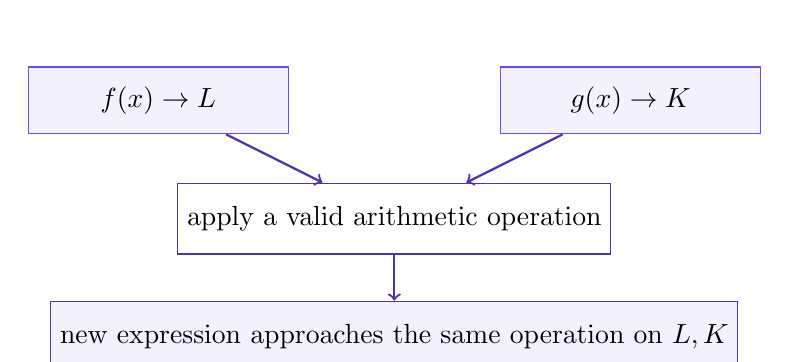
\begin{tikzpicture}
\node[draw=novelPurple,fill=novelPurpleLight,minimum width=3.3cm,minimum height=.85cm] (fx) at (-3,1.5) {$f(x)\to L$};
\node[draw=novelPurple,fill=novelPurpleLight,minimum width=3.3cm,minimum height=.85cm] (gx) at (3,1.5) {$g(x)\to K$};
\node[draw=novelPurpleDark,fill=white,minimum width=5cm,minimum height=.9cm] (op) at (0,0) {apply a valid arithmetic operation};
\node[draw=novelPurpleDark,fill=novelPurpleLight,minimum width=8cm,minimum height=.9cm] (ans) at (0,-1.5) {new expression approaches the same operation on $L,K$};
\draw[->,novelPurpleDark,thick] (fx)--(op);\draw[->,novelPurpleDark,thick] (gx)--(op);\draw[->,novelPurpleDark,thick](op)--(ans);
\end{tikzpicture}
\end{center}

\begin{notebox}{What Must Be Checked First}
Before applying a property, identify the target $x\to c$ and verify that the needed component limits exist. For a quotient, also verify that the denominator limit is not zero. For an even root, verify that nearby inputs remain in the real domain. These conditions are part of the mathematics, not optional footnotes.
\end{notebox}

\newpage
\subsection*{The Two Foundation Properties}

\begin{theorybox}{Constant Property}
For any constant $b$,
\[
\lim_{x\to c}b=b.
\]
The output never changes. No matter which nearby input is chosen, the function is already exactly at $b$.
\end{theorybox}

\example{A constant function.}
Evaluate $\lim_{x\to7}(-4)$.

\solution The function outputs $-4$ for every input, so it certainly approaches $-4$:
\[\boxed{-4}.\]

\begin{theorybox}{Identity Property}
\[
\lim_{x\to c}x=c.
\]
As the input $x$ moves closer to $c$, the output of the identity function $f(x)=x$ is the same number and therefore also moves closer to $c$.
\end{theorybox}

\example{The input itself.}
Evaluate $\lim_{x\to-3}x$.

\solution Values such as $-2.9,-2.99,-3.01$ approach $-3$, so
\[\boxed{-3}.\]

\begin{skillbox}{Why These Two Matter}
Every polynomial is built from constants and copies of $x$ using addition and multiplication. Once the arithmetic properties are established, polynomial limits follow automatically.
\end{skillbox}

\newpage
\subsection*{Sum and Difference Properties}

\begin{theorybox}{Statement and Meaning}
If $\lim_{x\to c}f(x)=L$ and $\lim_{x\to c}g(x)=K$, then
\[
\lim_{x\to c}[f(x)+g(x)]=L+K,
\qquad
\lim_{x\to c}[f(x)-g(x)]=L-K.
\]
Nearby sums approach the sum of the approached values; nearby differences approach their difference.
\end{theorybox}

\example{Using supplied component limits.}
Suppose $\lim_{x\to2}f(x)=5$ and $\lim_{x\to2}g(x)=-1$. Find
\[
\lim_{x\to2}[f(x)+g(x)].
\]

\solution
Name the property, then substitute the component limits:
\[
\lim_{x\to2}[f(x)+g(x)]
=\lim_{x\to2}f(x)+\lim_{x\to2}g(x)
=5+(-1)=\boxed4.
\]

\example{A difference with careful signs.}
Using the same information, find $\lim_{x\to2}[g(x)-f(x)]$.

\solution
\[
\lim[g(x)-f(x)]=K-L=-1-5=\boxed{-6}.
\]
The order of subtraction must be preserved.

\begin{notebox}{Common Error}
The sum property cannot rescue a missing component limit. If $\lim f$ does not exist and $\lim g$ exists, the property does not justify splitting the expression. Occasionally cancellation may make $f+g$ have a limit, but that requires analyzing the combined expression directly.
\end{notebox}

\newpage
\subsection*{Constant Multiple Property}

\begin{theorybox}{Statement and Meaning}
For a fixed real number $a$,
\[
\lim_{x\to c}[a f(x)]=a\lim_{x\to c}f(x)=aL.
\]
Multiplying every nearby output by $a$ scales the approached output by the same factor. A negative factor also reflects the values across the horizontal axis.
\end{theorybox}

\example{Scaling a known limit.}
If $\lim_{x\to4}f(x)=-3$, find $\lim_{x\to4}7f(x)$.

\solution
\[
\lim_{x\to4}7f(x)=7\lim_{x\to4}f(x)=7(-3)=\boxed{-21}.
\]

\example{Combining two properties.}
If $\lim f=2$ and $\lim g=5$ as $x\to c$, find
\[
\lim_{x\to c}[3f(x)-2g(x)+4].
\]

\solution
Apply constant multiple, difference, sum, and constant properties:
\[
3(2)-2(5)+4=6-10+4=\boxed0.
\]

\begin{skillbox}{Structure Reading}
Read from the largest operations inward. The expression is a sum of three terms: $3f(x)$, $-2g(x)$, and $4$. Evaluate the limit of each term, then add.
\end{skillbox}

\newpage
\subsection*{Product Property}

\begin{theorybox}{Statement and Meaning}
If $f(x)\to L$ and $g(x)\to K$, then
\[
f(x)g(x)\to LK.
\]
When both factors approach finite numbers, small changes in the factors create only small changes in their product.
\end{theorybox}

\example{Product of two known limits.}
If $\lim_{x\to1}f(x)=-2$ and $\lim_{x\to1}g(x)=6$, find
\[
\lim_{x\to1}f(x)g(x).
\]

\solution
\[
\lim f(x)g(x)=(\lim f)(\lim g)=(-2)(6)=\boxed{-12}.
\]

\example{A polynomial built from products and sums.}
Evaluate $\lim_{x\to3}(2x^2-5x+1)$ using properties.

\solution
\[
\begin{aligned}
\lim_{x\to3}(2x^2-5x+1)
&=2(\lim x)(\lim x)-5\lim x+1\\
&=2(3)(3)-5(3)+1\\
&=18-15+1=\boxed4.
\end{aligned}
\]

\begin{notebox}{Zero Product Caution}
If one finite factor approaches 0 and the other approaches a finite number, the product approaches 0. But $0\cdot\infty$ is an indeterminate form; the finite-limit product property does not apply to it.
\end{notebox}

\newpage
\subsection*{Quotient Property and Its Essential Restriction}

\begin{theorybox}{Statement}
If $f(x)\to L$, $g(x)\to K$, and $K\ne0$, then
\[
\lim_{x\to c}\frac{f(x)}{g(x)}=\frac{L}{K}.
\]
The condition $K\ne0$ matters because division is not stable near zero: a tiny denominator can create an enormous output or opposite signs on opposite sides.
\end{theorybox}

\example{A valid quotient-property application.}
If $\lim f=8$ and $\lim g=-2$, then
\[
\lim\frac{f(x)}{g(x)}=\frac8{-2}=\boxed{-4}.
\]

\example{Direct substitution into a rational function.}
Evaluate $\lim_{x\to2}\frac{x^2+3}{x+4}$.

\solution
The denominator limit is $2+4=6\ne0$, so the quotient property applies:
\[
\frac{2^2+3}{2+4}=\frac76.
\]

\example{Why a zero denominator stops the property.}
Consider $\lim_{x\to0}\frac{x}{x}$. Substitution gives $0/0$, but the nearby expression equals 1 and the limit is 1. By contrast, $\lim_{x\to0}1/x$ is unbounded and its two-sided limit does not exist. Therefore “denominator limit $=0$” does not determine the answer; it tells us the quotient property is unavailable.

\begin{skillbox}{Required Sentence}
“Because the denominator approaches a nonzero value, the quotient property applies.” If the denominator approaches zero, stop and choose a different analysis.
\end{skillbox}

\newpage
\subsection*{Power and Root Properties}

\begin{theorybox}{Powers}
For a positive integer $n$, if $f(x)\to L$, then
\[
\lim_{x\to c}[f(x)]^n=L^n.
\]
This follows from applying the product property repeatedly.
\end{theorybox}

\example{Power of a function.}
If $\lim_{x\to5}f(x)=-2$, find $\lim_{x\to5}[f(x)]^4$.

\solution $(-2)^4=\boxed{16}$. Parentheses matter: $(-2)^4$ is positive.

\begin{theorybox}{Roots and Domain Conditions}
For an odd root, $\sqrt[n]{y}$ is continuous for every real $y$. For an even root, the real-valued function requires $y\ge0$. Thus
\[
\lim_{x\to c}\sqrt[n]{f(x)}=\sqrt[n]{L}
\]
provided the nearby inputs lie in the root's real domain.
\end{theorybox}

\example{An odd root.}
\[
\lim_{x\to-1}\sqrt[3]{2x-6}=\sqrt[3]{-8}=\boxed{-2}.
\]

\example{An even root at an endpoint.}
For $f(x)=\sqrt{x-2}$, the two-sided real limit at 2 is not defined because there are no domain points immediately to the left. The correct endpoint statement is
\[
\lim_{x\to2^+}\sqrt{x-2}=0.
\]

\newpage
\subsection*{Composition Property: Outside Follows Inside}

\begin{theorybox}{Statement}
If $g(x)\to L$ as $x\to c$ and the outer function $f$ is continuous at $L$, then
\[
\lim_{x\to c}f(g(x))=f\left(\lim_{x\to c}g(x)\right)=f(L).
\]
The input of the outer function is not $x$; it is the entire inner output $g(x)$.
\end{theorybox}

\example{Square root of an inner expression.}
Evaluate $\lim_{x\to1}\sqrt{x^2+8}$.

\solution
First, $x^2+8\to9$. The square-root function is continuous at 9, so
\[
\sqrt{x^2+8}\to\sqrt9=\boxed3.
\]

\example{Trigonometric composition.}
\[
\lim_{x\to\pi/6}\sin(3x)
=\sin\left(3\cdot\frac\pi6\right)
=\sin\frac\pi2=\boxed1.
\]

\example{Composition where continuity fails.}
Let $f(u)=1/u$ and suppose $g(x)\to0$. Since $f$ is not continuous at 0, we cannot conclude that $f(g(x))\to f(0)$. In fact, $f(0)$ is undefined, and the limit depends on how $g(x)$ approaches zero.

\begin{notebox}{Inside-Outside Annotation}
Circle the inner expression, compute its limit, then ask whether the outer function is continuous at that new input. This prevents substituting into the wrong layer.
\end{notebox}

\newpage
\subsection*{Piecewise Functions: Properties Do Not Replace One-Sided Limits}

\begin{theorybox}{At a Boundary Point}
When a formula changes at $x=c$, use the rule valid for $x<c$ to find the left-hand limit and the rule valid for $x>c$ to find the right-hand limit. The equality symbol in the definition decides $f(c)$, but it does not decide either approached value.
\end{theorybox}

\example{Matching pieces.}
Let
\[
f(x)=\begin{cases}2x+1,&x<3,\\x+4,&x\ge3.\end{cases}
\]
Then
\[
\lim_{x\to3^-}f(x)=2(3)+1=7,
\qquad
\lim_{x\to3^+}f(x)=3+4=7.
\]
Therefore $\lim_{x\to3}f(x)=\boxed7$, and $f(3)=7$, so $f$ is continuous at 3.

\example{Nonmatching pieces.}
For
\[
g(x)=\begin{cases}x^2,&x<2,\\3x-1,&x\ge2,\end{cases}
\]
the left-hand limit is 4 and the right-hand limit is 5. Hence the two-sided limit is $\boxed{\mathrm{DNE}}$, even though $g(2)=5$ is defined.

\example{Finding a parameter for continuity.}
If
\[
h(x)=\begin{cases}kx+2,&x<1,\\5,&x\ge1,\end{cases}
\]
continuity at 1 requires $k(1)+2=5$, so $\boxed{k=3}$.

\begin{skillbox}{Boundary Checklist}
Left rule $\to$ left limit. Right rule $\to$ right limit. Compare them. Only after the limit is known should you compare it with the actual value.
\end{skillbox}

\newpage
\subsection*{Direct Substitution: The Final Consequence}

\begin{bigideabox}{Why Substitution Works}
Direct substitution is not a separate magic rule. It is the cumulative result of continuity and the limit properties. Constants and $x$ have the expected limits; sums, products, powers, valid quotients, roots, and compositions preserve those limits. Therefore a function assembled from continuous pieces is continuous wherever all operations are defined.
\end{bigideabox}

\begin{theorybox}{Four-Step Written Solution}
\begin{enumerate}
\item Identify the function family and its domain near $c$.
\item Check that no denominator, root, or logarithm condition fails.
\item State that the function is continuous at $c$.
\item Substitute and simplify carefully.
\end{enumerate}
\end{theorybox}

\example{A complete mixed example.}
Evaluate
\[
\lim_{x\to2}\frac{\sqrt{x^2+12}+3x}{x+1}.
\]

\solution
The polynomial expressions are continuous, the square-root input approaches $16>0$, and the denominator approaches $3\ne0$. Therefore all required properties apply:
\[
\begin{aligned}
\lim_{x\to2}\frac{\sqrt{x^2+12}+3x}{x+1}
&=\frac{\sqrt{2^2+12}+3(2)}{2+1}\\
&=\frac{4+6}{3}=\boxed{\frac{10}{3}}.
\end{aligned}
\]

\example{A diagnostic failure.}
For $\lim_{x\to2}\frac{x^2-4}{x-2}$, the denominator condition fails and direct substitution yields $0/0$. We do not conclude DNE. We record the indeterminate form and move to Topic 1.6, where factoring reveals the removable factor.

\begin{notebox}{Property Decision Map}
Finite component limits? Apply arithmetic properties. Quotient denominator nonzero? Divide. Outer function continuous at the inner limit? Compose. Piecewise boundary? Compare sides. Any condition fails? Stop; diagnose instead of forcing substitution.
\end{notebox}

\newpage
\subsection*{1.5 AP-Style Mastery Set with Fully Explained Answers}

\example{Interpreting a limit table.}
Given
\[
\begin{array}{c|ccc}
&\lim f(x)&\lim g(x)&\lim h(x)\\\hline
x\to2&-1&4&0
\end{array}
\]
find $\lim_{x\to2}[f(x)^2+3g(x)]$.

\solution The power, constant multiple, and sum properties give
\[
(-1)^2+3(4)=1+12=\boxed{13}.
\]

\example{Recognizing an invalid request.}
Can the same table determine $\lim_{x\to2}g(x)/h(x)$?

\solution No. The denominator approaches 0, so the quotient property does not apply. The table does not provide enough information about signs or relative rates to determine the quotient.

\example{Solving backward from a limit.}
Suppose $\lim_{x\to c}f(x)=3$ and
\[
\lim_{x\to c}[2f(x)+kg(x)]=14,
\qquad \lim_{x\to c}g(x)=4.
\]
Find $k$.

\solution
\[
2(3)+k(4)=14\implies6+4k=14\implies\boxed{k=2}.
\]

\example{A nested expression.}
If $\lim f=2$ and $\lim g=5$, find
\[
\lim\sqrt{[f(x)]^2+g(x)}.
\]

\solution The inside approaches $2^2+5=9$. Since square root is continuous at 9, the whole expression approaches $\sqrt9=\boxed3$.

\example{Explaining rather than calculating.}
Why is $\lim_{x\to1}\frac{x^2+1}{x^2+2}=\frac23$?

\solution Polynomials are continuous, the denominator value at 1 is $3\ne0$, and a quotient of continuous functions is continuous where the denominator is nonzero. Therefore direct substitution is justified and gives $2/3$.

\begin{skillbox}{What Mastery Looks Like}
A strong student can name the property, state its condition, show the component limits, and explain why the condition is satisfied. Merely writing the final substituted number is not a complete conceptual solution.
\end{skillbox}
 
\newpage

%
%
%
\section{Determining Limits Using Algebraic Manipulation}

Sometimes direct substitution leads to an indeterminate form such as
\[
\frac{0}{0}.
\]
In that case, the limit may still exist, but we need to rewrite the expression.

\begin{theorybox}{Most Common Algebraic Techniques}
\begin{enumerate}
    \item factoring and canceling common factors
    \item rationalizing with a conjugate
    \item combining fractions over a common denominator
    \item simplifying complex fractions
\end{enumerate}
\end{theorybox}

\subsection{Factoring}

\example{Factoring out a common factor.}

Find:
\[
\lim_{x\to 1}\frac{x^3-1}{x-1}.
\]

\bigskip

\solution

Direct substitution gives
\[
\frac{1^3-1}{1-1}=\frac00,
\]
so we factor:
\[
x^3-1=(x-1)(x^2+x+1).
\]
Thus
\[
\frac{x^3-1}{x-1}=x^2+x+1,\qquad x\neq 1.
\]
Now take the limit:
\[
\lim_{x\to 1}(x^2+x+1)=1+1+1=3.
\]

\[
\boxed{3}
\]

\subsection{Rationalizing}

\example{Rationalizing a radical expression.}

Find:
\[
\lim_{x\to 0}\frac{x}{\sqrt{x+1}-1}.
\]

\bigskip

\solution

Direct substitution gives
\[
\frac{0}{0},
\]
so multiply numerator and denominator by the conjugate:
\[
\frac{x}{\sqrt{x+1}-1}\cdot\frac{\sqrt{x+1}+1}{\sqrt{x+1}+1}
=
\frac{x(\sqrt{x+1}+1)}{(x+1)-1}.
\]
The denominator simplifies to $x$, so
\[
\frac{x(\sqrt{x+1}+1)}{x}=\sqrt{x+1}+1,\qquad x\neq 0.
\]
Now substitute:
\[
\lim_{x\to 0}(\sqrt{x+1}+1)=\sqrt{1}+1=2.
\]

\[
\boxed{2}
\]

\subsection{Combining Fractions}

\example{Common denominator method.}

Find:
\[
\lim_{x\to 0}\frac{\frac{1}{x+2}-\frac12}{x}.
\]

\bigskip

\solution

First combine the terms in the numerator:
\[
\frac{1}{x+2}-\frac12
=
\frac{2-(x+2)}{2(x+2)}
=
\frac{-x}{2(x+2)}.
\]
So
\[
\frac{\frac{1}{x+2}-\frac12}{x}
=
\frac{-x}{2(x+2)}\cdot \frac{1}{x}
=
-\frac{1}{2(x+2)}.
\]
Now substitute $x=0$:
\[
-\frac{1}{2(2)}=-\frac14.
\]

\[
\boxed{-\frac14}
\]

\bigskip

\apcheckpoint{If direct substitution gives $\frac00$, do not conclude the limit does not exist. Instead, look for algebraic simplification.}

\newpage

%
%
%
\section{Selecting Procedures for Determining Limits}

\begin{skillbox}{Strategy Ladder}
When evaluating a limit, use this decision order:
\begin{enumerate}
    \item \textbf{Try direct substitution.}
    \item If you get a real number, you are done.
    \item If you get $\frac00$, simplify algebraically.
    \item If the expression is bounded by two simpler expressions, consider the Squeeze Theorem.
    \item If the function is piecewise or graph-based, compare left- and right-hand behavior.
    \item If the variable goes to $\infty$ or $-\infty$, analyze end behavior.
\end{enumerate}
\end{skillbox}

\example{Choosing the right procedure.}

State the best method first, then evaluate:
\[
\lim_{x\to 4}\frac{x^2-16}{x-4}.
\]

\bigskip

\solution

Direct substitution gives
\[
\frac{16-16}{4-4}=\frac00,
\]
so the best method is \textbf{factoring}.

\[
x^2-16=(x-4)(x+4).
\]
Then
\[
\frac{x^2-16}{x-4}=x+4,\qquad x\neq 4.
\]
Now substitute:
\[
\lim_{x\to 4}(x+4)=8.
\]

\[
\boxed{8}
\]

\bigskip

\example{Choosing direct substitution instead.}

Evaluate:
\[
\lim_{x\to -2}(3x^3-5x+7).
\]

\bigskip

\solution

This is a polynomial, so direct substitution is the best method:
\[
3(-2)^3-5(-2)+7
=
3(-8)+10+7
=
-24+17=-7.
\]

\[
\boxed{-7}
\]

\newpage

%
%
%
\section{Determining Limits Using the Squeeze Theorem}

\begin{theorybox}{Squeeze Theorem}
If
\[
g(x)\le f(x)\le h(x)
\]
for all $x$ near $c$ (except possibly at $c$), and if
\[
\lim_{x\to c}g(x)=\lim_{x\to c}h(x)=L,
\]
then
\[
\lim_{x\to c}f(x)=L.
\]
\end{theorybox}

\begin{theorybox}{A Classic Bounding Fact}
Because
\[
-1\le \sin\theta \le 1
\]
for all real $\theta$, we often multiply by a quantity involving $x$ to create useful bounds.
\end{theorybox}

\example{A classic Squeeze Theorem problem.}

Find:
\[
\lim_{t\to 0} t^2\sin\!\left(\frac{1}{t}\right).
\]

\bigskip

\solution

Since
\[
-1\le \sin\left(\frac1t\right)\le 1,
\]
multiply everything by $t^2$.
Because $t^2\ge 0$ for all real $t$, the inequality direction stays the same:
\[
-t^2\le t^2\sin\left(\frac1t\right)\le t^2.
\]
Now take limits:
\[
\lim_{t\to 0}(-t^2)=0
\qquad\text{and}\qquad
\lim_{t\to 0}t^2=0.
\]
Therefore, by the Squeeze Theorem,
\[
\lim_{t\to 0} t^2\sin\left(\frac1t\right)=0.
\]

\[
\boxed{0}
\]

\bigskip
\newpage
\example{A trigonometric squeeze-based fact.}

A standard special limit is
\[
\lim_{x\to 0}\frac{\sin x}{x}=1.
\]
Use it to find:
\[
\lim_{x\to 0}\frac{\sin 4x}{x}.
\]

\bigskip

\solution

Rewrite the expression:
\[
\frac{\sin 4x}{x}
=
4\cdot \frac{\sin 4x}{4x}.
\]
As $x\to 0$, we also have $4x\to 0$, so
\[
\lim_{x\to 0}\frac{\sin 4x}{4x}=1.
\]
Therefore
\[
\lim_{x\to 0}\frac{\sin 4x}{x}
=
4(1)=4.
\]

\[
\boxed{4}
\]

\bigskip

\begin{theorybox}{Two Special Trigonometric Limits}
\[
\lim_{x\to 0}\frac{\sin x}{x}=1
\qquad\text{and}\qquad
\lim_{x\to 0}\frac{1-\cos x}{x}=0.
\]
\end{theorybox}

\newpage

%
%
%
\section{Connecting Multiple Representations of Limits}

\begin{theorybox}{Same Idea, Different Forms}
A limit can be represented:
\begin{itemize}
    \item graphically
    \item numerically (table)
    \item algebraically
    \item verbally
\end{itemize}
A strong AP student should be able to move smoothly between all four.
\end{theorybox}

\example{Connecting a graph, table, and formula.}

Suppose a function satisfies:
\[
f(x)=\frac{x^2-9}{x-3},\qquad x\neq 3.
\]
Describe the limit as $x\to 3$ in three ways.

\bigskip

\solution

\textbf{Algebraic view:}
\[
\frac{x^2-9}{x-3}=\frac{(x-3)(x+3)}{x-3}=x+3,\qquad x\neq 3.
\]
So
\[
\lim_{x\to 3}f(x)=6.
\]

\textbf{Numerical view:}
Values of $x$ near $3$ produce outputs near $6$.

\textbf{Graphical view:}
The graph follows the line $y=x+3$ with a hole at $(3,6)$, so the graph approaches $6$ as $x\to 3$.

\textbf{Verbal view:}
As the input approaches $3$, the output approaches $6$.

\bigskip

\apcheckpoint{A removable hole is one of the best examples for teaching that a limit depends on approach behavior, not just on whether the point itself is filled in.}

%
%
%
\section{Exploring Types of Discontinuities}

\begin{theorybox}{Three Common Types of Discontinuity}
\begin{enumerate}
    \item \textbf{Removable discontinuity:} the graph has a hole; the limit exists.
    \item \textbf{Jump discontinuity:} left- and right-hand limits are finite but unequal.
    \item \textbf{Infinite discontinuity:} the function grows without bound near a point.
\end{enumerate}
\end{theorybox}

\subsection{Visual Classification}

\begin{center}
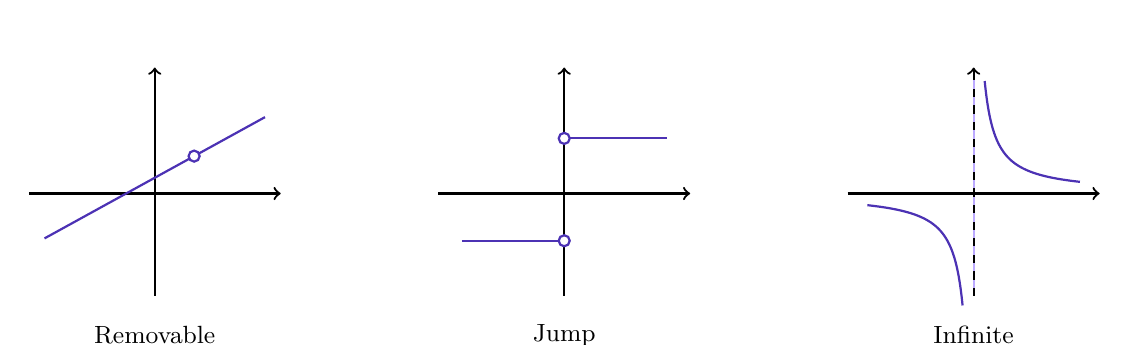
\begin{tikzpicture}[scale=1]
%
\begin{scope}[shift={(-5.2,0)}]
\draw[->, thick] (-1.6,0) -- (1.6,0);
\draw[->, thick] (0,-1.3) -- (0,1.6);
\draw[novelPurpleDark, thick, domain=-1.4:1.4, samples=120] plot (\x,{0.55*\x+0.2});
\draw[novelPurpleDark, fill=white, thick] (0.5,0.475) circle (0.07);
\node at (0,-1.8) {\small Removable};
\end{scope}

%
\begin{scope}[shift={(0,0)}]
\draw[->, thick] (-1.6,0) -- (1.6,0);
\draw[->, thick] (0,-1.3) -- (0,1.6);
\draw[novelPurpleDark, thick] (-1.3,-0.6) -- (0,-0.6);
\draw[novelPurpleDark, thick] (0,0.7) -- (1.3,0.7);
\draw[novelPurpleDark, fill=white, thick] (0,-0.6) circle (0.07);
\draw[novelPurpleDark, fill=white, thick] (0,0.7) circle (0.07);
\node at (0,-1.8) {\small Jump};
\end{scope}

%
\begin{scope}[shift={(5.2,0)}]
\draw[->, thick] (-1.6,0) -- (1.6,0);
\draw[->, thick] (0,-1.3) -- (0,1.6);
\draw[dashed, novelPurpleLine, thick] (0,-1.2) -- (0,1.5);
\draw[novelPurpleDark, thick, domain=-1.35:-0.14, samples=120] plot (\x,{0.2/(\x)});
\draw[novelPurpleDark, thick, domain=0.14:1.35, samples=120] plot (\x,{0.2/(\x)});
\node at (0,-1.8) {\small Infinite};
\end{scope}
\end{tikzpicture}
\end{center}

\example{Classifying discontinuities.}

Classify the discontinuity at the indicated point.

\begin{enumerate}
    \item $\ds f(x)=\frac{x^2-4}{x-2}$ at $x=2$
    \item $\ds g(x)=\frac{|x|}{x}$ at $x=0$
    \item $\ds h(x)=\frac{1}{x^2}$ at $x=0$
\end{enumerate}

\bigskip

\solution

\textbf{1.}
\[
\frac{x^2-4}{x-2}=\frac{(x-2)(x+2)}{x-2}=x+2,\qquad x\neq 2.
\]
The graph has a hole at $x=2$, so this is a \textbf{removable discontinuity}.

\textbf{2.} The left-hand limit is $-1$ and the right-hand limit is $1$, so the function has a \textbf{jump discontinuity}.

\textbf{3.} As $x\to 0$, the function grows without bound, so this is an \textbf{infinite discontinuity}.

\newpage

%
%
%
\section{Defining Continuity at a Point}

\begin{theorybox}{Continuity at a Point}
A function $f$ is continuous at $x=c$ if all three conditions are true:
\begin{enumerate}
    \item $f(c)$ is defined.
    \item $\lim\limits_{x\to c}f(x)$ exists.
    \item $\lim\limits_{x\to c}f(x)=f(c)$.
\end{enumerate}
\end{theorybox}

\example{Testing continuity with the three-condition definition.}

Determine whether
\[
f(x)=
\begin{cases}
\dfrac{x^2-x-2}{x-2}, & x\neq 2,\\[0.6em]
1, & x=2
\end{cases}
\]
is continuous at $x=2$.

\bigskip

\solution

\textbf{Condition 1:} $f(2)$ is defined, and
\[
f(2)=1.
\]

\textbf{Condition 2:} For $x\neq 2$,
\[
\frac{x^2-x-2}{x-2}
=
\frac{(x-2)(x+1)}{x-2}=x+1.
\]
So
\[
\lim_{x\to 2}f(x)=\lim_{x\to 2}(x+1)=3.
\]

\textbf{Condition 3:} Compare:
\[
\lim_{x\to 2}f(x)=3
\qquad\text{but}\qquad
f(2)=1.
\]
Since these are not equal, the function is \textbf{not continuous} at $x=2$.

\bigskip

\begin{notebox}{Fast Continuity Test}
Whenever a function is built from standard continuous functions and no domain restriction is violated, it is continuous automatically. But for piecewise functions and rational functions at excluded values, use the 3-condition definition carefully.
\end{notebox}

%
%
%
\newpage
\section{Confirming Continuity over an Interval}

\subsection{Open Intervals}

A function is continuous on an open interval $(a,b)$ if it is continuous at every point in that interval.

\subsection{Closed Intervals}

\begin{theorybox}{Continuity on a Closed Interval}
A function is continuous on $[a,b]$ if:
\begin{enumerate}
    \item it is continuous on $(a,b)$,
    \item $\lim\limits_{x\to a^+}f(x)=f(a)$,
    \item $\lim\limits_{x\to b^-}f(x)=f(b)$.
\end{enumerate}
\end{theorybox}

\begin{theorybox}{One-Sided Limits}
\[
\lim_{x\to c^-}f(x)=L
\quad\text{means the left-hand limit}
\]
and
\[
\lim_{x\to c^+}f(x)=L
\quad\text{means the right-hand limit.}
\]
A two-sided limit exists exactly when the left-hand and right-hand limits both exist and are equal.
\end{theorybox}

\example{Continuity on a closed interval.}

Discuss the continuity of
\[
f(x)=\sqrt{1-x^2}.
\]

\bigskip

\solution

The domain is
\[
-1\le x\le 1,
\]
so the function is defined on the closed interval $[-1,1]$.

Inside the interval, the square-root function composed with $1-x^2$ is continuous wherever defined, so $f$ is continuous on $(-1,1)$.

Now check the endpoints:
\[
\lim_{x\to -1^+}\sqrt{1-x^2}=0=f(-1),
\]
and
\[
\lim_{x\to 1^-}\sqrt{1-x^2}=0=f(1).
\]

Therefore, $f$ is continuous on
\[
\boxed{[-1,1]}.
\]

\newpage

%
%
%
\section{Removing Discontinuities}

\begin{theorybox}{Removable Discontinuity Idea}
If a limit exists at $x=c$ but the function is either undefined there or defined incorrectly there, then the discontinuity can be removed by redefining the function value to equal the limit.
\end{theorybox}

\example{Making a function continuous by redefining one point.}

Find a value of $k$ that makes
\[
f(x)=
\begin{cases}
\dfrac{x^2-9}{x-3}, & x\neq 3,\\[0.6em]
k, & x=3
\end{cases}
\]
continuous at $x=3$.

\bigskip

\solution

To be continuous at $x=3$, we need
\[
k=\lim_{x\to 3}\frac{x^2-9}{x-3}.
\]
Factor:
\[
\frac{x^2-9}{x-3}
=
\frac{(x-3)(x+3)}{x-3}=x+3,\qquad x\neq 3.
\]
So
\[
\lim_{x\to 3}\frac{x^2-9}{x-3}
=
\lim_{x\to 3}(x+3)=6.
\]
Thus the required value is
\[
\boxed{k=6}.
\]

\bigskip

\apcheckpoint{This is one of the most important continuity templates in AP Calculus: simplify first, find the limit, then define the missing point to match it.}

%
%
%
\newpage
\section{Infinite Limits and Vertical Asymptotes}

\begin{theorybox}{Infinite Limits}
If the values of $f(x)$ increase without bound as $x$ approaches $c$, we write
\[
\lim_{x\to c}f(x)=\infty.
\]
If the values decrease without bound, we write
\[
\lim_{x\to c}f(x)=-\infty.
\]
\end{theorybox}

\begin{theorybox}{Vertical Asymptotes}
If at least one of
\[
\lim_{x\to c^-}f(x),\qquad \lim_{x\to c^+}f(x)
\]
is $\infty$ or $-\infty$, then the line
\[
x=c
\]
is a vertical asymptote.
\end{theorybox}

\example{Finding a vertical asymptote.}

Determine the behavior of
\[
f(x)=\frac{1}{x-2}
\]
as $x\to 2^-$ and as $x\to 2^+$.

\bigskip

\solution

As $x\to 2^-$, the denominator $x-2$ is a very small negative number, so
\[
\frac{1}{x-2}\to -\infty.
\]

As $x\to 2^+$, the denominator $x-2$ is a very small positive number, so
\[
\frac{1}{x-2}\to \infty.
\]

Therefore,
\[
\lim_{x\to 2^-}\frac{1}{x-2}=-\infty,
\qquad
\lim_{x\to 2^+}\frac{1}{x-2}=\infty,
\]
and the graph has a vertical asymptote at
\[
\boxed{x=2}.
\]

\bigskip

\example{A rational function with a common factor.}

Determine all vertical asymptotes of
\[
f(x)=\frac{x^2+2x-8}{x^2-4}.
\]

\bigskip

\solution

Factor numerator and denominator:
\[
x^2+2x-8=(x+4)(x-2),
\qquad
x^2-4=(x+2)(x-2).
\]
So
\[
f(x)=\frac{(x+4)(x-2)}{(x+2)(x-2)}=\frac{x+4}{x+2},\qquad x\neq 2.
\]

The factor $x-2$ cancels, so $x=2$ is a hole, not a vertical asymptote.

The denominator of the simplified form is zero at $x=-2$, so
\[
x=-2
\]
is the vertical asymptote.

Thus the only vertical asymptote is
\[
\boxed{x=-2}.
\]

\newpage

%
%
%
\section{Limits at Infinity and Horizontal Asymptotes}

\begin{theorybox}{Limits at Infinity}
Limits at infinity describe how a function behaves as
\[
x\to \infty
\qquad\text{or}\qquad
x\to -\infty.
\]
These are end-behavior questions.
\end{theorybox}

\begin{theorybox}{Horizontal Asymptotes}
If
\[
\lim_{x\to\infty}f(x)=L
\quad\text{or}\quad
\lim_{x\to-\infty}f(x)=L,
\]
then the line
\[
y=L
\]
is a horizontal asymptote.
\end{theorybox}

\subsection{Rational Functions and End Behavior}

For rational functions, compare degrees:

\begin{itemize}
    \item If degree of numerator $<$ degree of denominator, then
    \[
    \lim_{x\to\pm\infty}f(x)=0.
    \]
    \item If degrees are equal, the limit is the ratio of leading coefficients.
    \item If degree of numerator $>$ degree of denominator, there is no horizontal asymptote.
\end{itemize}

\example{A zero horizontal asymptote.}

Find
\[
\lim_{x\to\infty}\frac{3x+1}{x^2+4}.
\]

\bigskip

\solution

The numerator has degree $1$, while the denominator has degree $2$. Since the denominator grows faster,
\[
\lim_{x\to\infty}\frac{3x+1}{x^2+4}=0.
\]
So the horizontal asymptote is
\[
\boxed{y=0}.
\]

\bigskip

\example{A ratio of leading coefficients.}

Find
\[
\lim_{x\to\infty}\frac{4x^2-7}{2x^2+5x+1}.
\]

\bigskip

\solution

The degrees are equal, so the limit is the ratio of leading coefficients:
\[
\lim_{x\to\infty}\frac{4x^2-7}{2x^2+5x+1}
=
\frac{4}{2}=2.
\]
Thus the horizontal asymptote is
\[
\boxed{y=2}.
\]

\bigskip

\example{Connecting horizontal asymptotes with graphs.}

Sketch the end behavior of a function satisfying
\[
\lim_{x\to\infty}f(x)=1
\qquad\text{and}\qquad
\lim_{x\to-\infty}f(x)=1.
\]

\bigskip

\solution

Both ends of the graph approach the line
\[
y=1.
\]
So $y=1$ is the horizontal asymptote.

\begin{center}
\begin{tikzpicture}
\begin{axis}[
    axis lines=middle,
    xmin=-5.3,xmax=5.3,
    ymin=-1.0,ymax=3.0,
    width=11.8cm,
    height=6.6cm,
    xtick={-4,-2,0,2,4},
    ytick={0,1,2},
    xlabel={$x$},
    ylabel={$y$},
    every axis x label/.style={at={(current axis.right of origin)}, anchor=west},
    every axis y label/.style={at={(current axis.above origin)}, anchor=south},
]
\addplot[dashed, novelPurpleLine, thick, domain=-5.2:5.2] {1};
\addplot[novelPurpleDark, very thick, domain=-5:5, samples=200] {1 + 1/(x^2+1)};
\end{axis}
\end{tikzpicture}
\end{center}

\newpage

%
%
%
\section{Applying the Intermediate Value Theorem}

\begin{bigideabox}{Big Idea}
A continuous graph cannot jump over an output value. If $f$ is continuous on $[a,b]$ and a number $N$ lies between $f(a)$ and $f(b)$, then at least one $c\in(a,b)$ satisfies $f(c)=N$.
\end{bigideabox}

\begin{theorybox}{The AP-Ready IVT Justification}
Every complete response must name all three ingredients:
\begin{enumerate}
    \item $f$ is continuous on the closed interval $[a,b]$;
    \item $N$ lies between $f(a)$ and $f(b)$;
    \item therefore, by the Intermediate Value Theorem, there exists at least one $c\in(a,b)$ such that $f(c)=N$.
\end{enumerate}
The theorem guarantees \emph{existence}, not the exact location, uniqueness, or the shape of the graph.
\end{theorybox}

\example{Guaranteeing a root.}
Let $f(x)=x^3+x-1$. Show that $f(x)=0$ has a solution in $(0,1)$.

\solution
Polynomials are continuous. Also, $f(0)=-1$ and $f(1)=1$. Since $0$ lies between $-1$ and $1$, the IVT guarantees a $c\in(0,1)$ with $f(c)=0$.

\bigskip
\example{Guaranteeing a target value from a table.}
A continuous function has $f(3)=-5$ and $f(4)=3$. Must $f(x)=2$ somewhere in $(3,4)$?

\solution
Yes. The target $2$ lies between $-5$ and $3$, so the IVT guarantees at least one $c\in(3,4)$ with $f(c)=2$.

\bigskip
\example{Could happen versus must happen.}
Suppose $f$ is continuous on $[4,8]$, with $f(4)=3$ and $f(8)=7$. Could $f(c)=-2$ for some $c\in(4,8)$? Must it?

\solution
It \emph{could} happen if the graph dips below $-2$, but the IVT does not guarantee it because $-2$ is not between the endpoint values $3$ and $7$.

\bigskip
\example{Counting the minimum number of zeros.}
For a continuous $f$, suppose
\[
\begin{array}{c|ccccc}
x&-5&1&3&8&14\\ \hline
f(x)&7&40&21&75&-100
\end{array}
\]
What is the minimum number of zeros on $[-5,14]$?

\solution
Only the interval $[8,14]$ has endpoint values with opposite signs. Thus the IVT guarantees at least one zero there. The minimum is $\boxed{1}$.

\bigskip
\example{Writing a complete AP justification.}
Show that $g(x)=\ln x+x$ takes the value $3$ on $[1,3]$.

\solution
The functions $\ln x$ and $x$ are continuous for $x>0$, so $g$ is continuous on $[1,3]$. We have $g(1)=1$ and $g(3)=3+\ln 3>3$. Since $3$ lies between these values, the IVT guarantees a $c\in(1,3)$ such that $g(c)=3$.

\begin{skillbox}{Common IVT Mistakes}
\begin{itemize}
    \item Checking endpoint values but never stating continuity.
    \item Claiming the solution is unique; the IVT only guarantees at least one.
    \item Using an open interval when the continuity hypothesis is needed on $[a,b]$.
    \item Saying a value is guaranteed when it is not between the endpoint outputs.
\end{itemize}
\end{skillbox}

\newpage

%
%
%
%
%
%
%
\newcommand{\method}[1]{\begin{notebox}{Method: What to Think Before Calculating}#1\end{notebox}}
\newcommand{\quickcheck}[2]{\textbf{#1}\quad #2\par\medskip}

\newpage
\section*{Deep-Dive Lesson Studios}
\addcontentsline{toc}{section}{Deep-Dive Lesson Studios}
\begin{skillbox}{How to Use These Studios}
Each studio revisits one lesson at a slower teaching pace. Read the decision rule first, cover the solution, and explain the reasoning aloud before checking the algebra. Every studio contains five worked examples and at least one representation-based checkpoint.
\end{skillbox}

\subsection*{Studio 1.1 --- Average Rate Becomes Instantaneous Rate}
\method{For an interval $[a,b]$, average rate is $\frac{f(b)-f(a)}{b-a}$. To describe rate at $a$, replace $b$ by $a+h$ and study what the secant slope approaches as $h\to0$. The limit is a number; the nearby secant slopes are evidence for that number.}
\quickcheck{Example 1.}{For $s(t)=t^2$, the average velocity on $[2,5]$ is $\frac{25-4}{3}=7$.}
\quickcheck{Example 2.}{On $[2,2.1]$, the slope is $\frac{2.1^2-2^2}{0.1}=4.1$. This is closer to the instantaneous velocity at $t=2$.}
\quickcheck{Example 3.}{On $[2,2+h]$, the slope is $\frac{(2+h)^2-4}{h}=4+h$, so the limiting slope is $4$.}
\quickcheck{Example 4.}{If temperature rises from $61^\circ$ to $73^\circ$ in 3 hours, the average rate is $4^\circ$/hour; it does not say the temperature rose at that rate at every instant.}
\quickcheck{Example 5.}{If $P(t)$ is population, $\frac{P(10.01)-P(10)}{0.01}$ estimates the instantaneous population growth rate at year 10, with units people/year.}
\begin{center}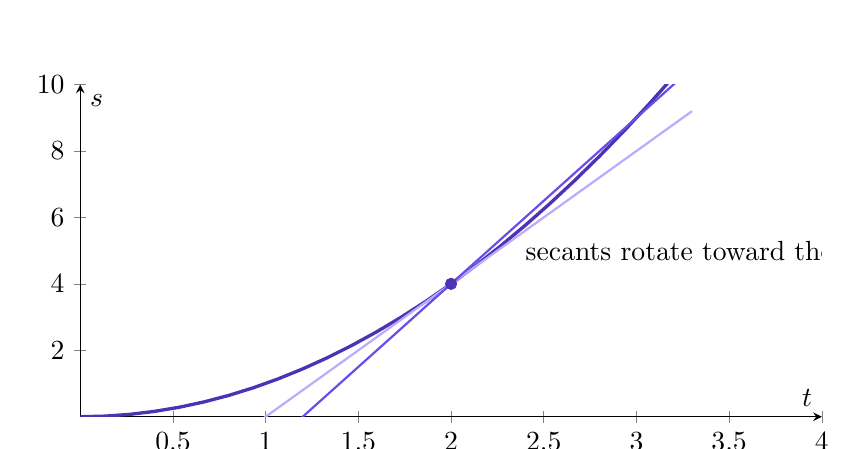
\begin{tikzpicture}\begin{axis}[width=11cm,height=5.8cm,axis lines=middle,xmin=0,xmax=4,ymin=0,ymax=10,xlabel={$t$},ylabel={$s$}]
\addplot[novelPurpleDark,very thick,domain=0:3.2]{x^2};
\addplot[novelPurpleLine,thick,domain=.8:3.3]{4*x-4};
\addplot[novelPurple,thick,domain=.8:3.3]{5*x-6};
\addplot[only marks,mark=*,novelPurpleDark] coordinates {(2,4)};
\node[anchor=west] at (axis cs:2.35,4.9){secants rotate toward the tangent};
\end{axis}\end{tikzpicture}\end{center}

\newpage
\subsection*{Studio 1.2 --- Limit Notation Says “Near,” Not “At”}
\method{Read $\lim_{x\to c}f(x)=L$ in three parts: input $x$ approaches $c$; output $f(x)$ approaches $L$; the value $f(c)$ may equal $L$, differ from $L$, or be undefined.}
\quickcheck{Example 1.}{$\lim_{x\to3}(2x-1)=5$ because outputs near $x=3$ are near 5.}
\quickcheck{Example 2.}{If a graph has a hole at $(2,4)$ and a filled point at $(2,7)$, then $\lim_{x\to2}f(x)=4$ but $f(2)=7$.}
\quickcheck{Example 3.}{If both sides approach $-1$ and there is no point at $x=5$, the limit still equals $-1$.}
\quickcheck{Example 4.}{If the left side approaches 2 and the right side approaches 6, write $\lim_{x\to c}f(x)=\mathrm{DNE}$, not 4.}
\quickcheck{Example 5.}{$\lim_{x\to c^-}$ means inputs smaller than $c$; $\lim_{x\to c^+}$ means inputs larger than $c$. The signs describe the input side, not the sign of the answer.}
\begin{skillbox}{Language Check}A limit is an approached output. A function value is an assigned output. Never replace “approaches” by “equals” unless continuity has been established.\end{skillbox}

\newpage
\subsection*{Studio 1.3 --- Reading Graphs in the Correct Order}
\method{At $x=c$, trace the curve from the left, then from the right. Record the two approached heights before looking at the filled point. A two-sided limit exists exactly when the two one-sided limits are the same finite or infinite behavior.}
\quickcheck{Example 1.}{Left height 3, right height 3, filled point 8: the limit is 3 and the function value is 8.}
\quickcheck{Example 2.}{Left height $-2$, right height 4: the two-sided limit does not exist.}
\quickcheck{Example 3.}{Both branches rise without bound near $x=1$: $\lim_{x\to1}f(x)=+\infty$.}
\quickcheck{Example 4.}{Left branch falls to $-\infty$ while the right rises to $+\infty$: the two-sided limit is DNE, although $x=1$ is a vertical asymptote.}
\quickcheck{Example 5.}{At an endpoint $x=a$ of a domain $[a,b]$, only the right-hand limit is relevant to right-continuity.}
\begin{center}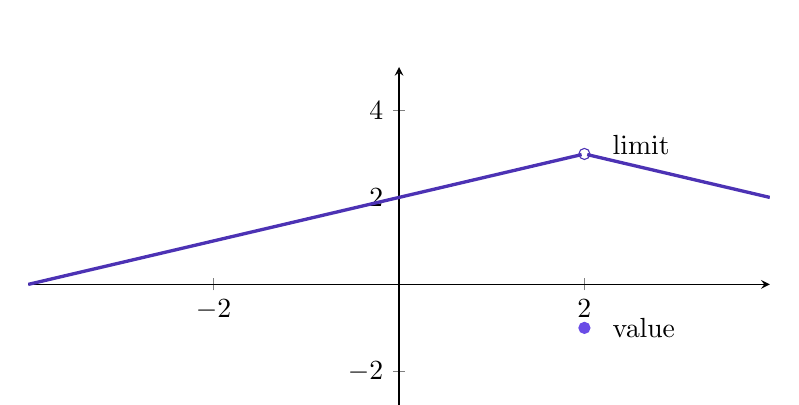
\begin{tikzpicture}\begin{axis}[width=11cm,height=6cm,axis lines=middle,xmin=-4,xmax=4,ymin=-3,ymax=5,xtick={-2,0,2},ytick={-2,0,2,4}]
\addplot[novelPurpleDark,very thick,domain=-4:1.97]{.5*x+2};
\addplot[novelPurpleDark,very thick,domain=2.03:4]{-.5*x+4};
\addplot[only marks,mark=o,mark options={fill=white},novelPurpleDark] coordinates {(2,3)};
\addplot[only marks,mark=*,novelPurple] coordinates {(2,-1)};
\node[anchor=west] at (axis cs:2.2,3.2){limit};\node[anchor=west] at (axis cs:2.2,-1){value};
\end{axis}\end{tikzpicture}\end{center}

\newpage
\subsection*{Studio 1.4 --- Tables Need Direction and Scale}
\method{Choose inputs on both sides of $c$ and increasingly close to $c$. Do not include only $x=c$. Compare stabilization from the left and right, and remember that rounded calculator output can hide disagreement or unbounded behavior.}
\quickcheck{Example 1.}{For $f(x)=\frac{x^2-9}{x-3}$, values at $2.9,2.99,3.01,3.1$ approach 6 because the expression equals $x+3$ when $x\ne3$.}
\quickcheck{Example 2.}{Values $1.9,1.99,2.01,2.1$ producing $4.8,4.98,5.02,5.2$ support a limit of 5.}
\quickcheck{Example 3.}{Left outputs near 2 and right outputs near 7 show DNE even if the table contains $f(c)=4$.}
\quickcheck{Example 4.}{Outputs $10,100,1000$ on both sides indicate $+\infty$, not a large finite limit.}
\quickcheck{Example 5.}{For $\sin x/x$, symmetric values near 0 approach 1; the missing value at 0 does not prevent the limit.}
\begin{theorybox}{A Strong Table}\centering
\begin{tabular}{c|cccccc}$x$&1.9&1.99&1.999&2.001&2.01&2.1\\\hline$f(x)$&4.8&4.98&4.998&5.002&5.02&5.2\end{tabular}
\par\medskip The inputs approach from both directions and the outputs close in on the same value.\end{theorybox}

\newpage
\subsection*{Studio 1.5 --- Limit Laws and Direct Substitution}
\method{First substitute. If every component is continuous at $c$ and no illegal operation occurs, the substituted value is the limit. The laws preserve sums, differences, constant multiples, products, quotients with nonzero denominator limit, powers, and appropriate roots.}
\quickcheck{Example 1.}{$\lim_{x\to2}(3x^2-5x+1)=12-10+1=3$.}
\quickcheck{Example 2.}{$\lim_{x\to1}\frac{x+4}{x^2+3}=\frac54$.}
\quickcheck{Example 3.}{$\lim_{x\to4}\sqrt{x+5}=3$ because the square-root function is continuous there.}
\quickcheck{Example 4.}{If $\lim f=2$ and $\lim g=-3$, then $\lim(4f-g)=4(2)-(-3)=11$.}
\quickcheck{Example 5.}{If $\lim g=0$, the quotient law cannot justify $\lim f/g$; the result might be finite, infinite, or DNE.}
\begin{skillbox}{Decision Signal}$0/0$ is not an answer. It is an indeterminate form telling you that direct substitution has revealed hidden algebra that must be simplified.\end{skillbox}

\newpage
\subsection*{Studio 1.6 --- Algebraic Manipulation Removes the Obstacle}
\method{After obtaining $0/0$, identify the structure: factor polynomials, rationalize radicals, or combine complex fractions. Cancel only factors, never terms. Then substitute into the simplified expression.}
\quickcheck{Example 1.}{$\lim_{x\to4}\frac{x^2-16}{x-4}=\lim(x+4)=8$.}
\quickcheck{Example 2.}{$\lim_{x\to-2}\frac{x^2+5x+6}{x+2}=\lim(x+3)=1$.}
\quickcheck{Example 3.}{$\lim_{x\to0}\frac{\sqrt{x+9}-3}{x}=\lim\frac1{\sqrt{x+9}+3}=\frac16$.}
\quickcheck{Example 4.}{$\lim_{x\to0}\frac{\frac1{x+1}-1}{x}=\lim\frac{-1}{x+1}=-1$.}
\quickcheck{Example 5.}{$\lim_{x\to0}\frac{\sin(5x)}{x}=5\lim\frac{\sin(5x)}{5x}=5$.}
\begin{notebox}{Cancellation Warning}$\frac{x^2-16}{x-4}=\frac{(x-4)(x+4)}{x-4}$ permits cancellation for $x\ne4$. The simplified function shares the original function's nearby behavior, not necessarily its value at 4.\end{notebox}

\newpage
\subsection*{Studio 1.7 --- Procedure Selection Is the Main Skill}
\method{Use this order: substitute $\rightarrow$ classify the result $\rightarrow$ simplify if $0/0$ $\rightarrow$ analyze signs if nonzero/0 $\rightarrow$ compare one-sided limits if a rule changes $\rightarrow$ use numerical/graphical evidence only when exact algebra is unavailable.}
\quickcheck{Example 1.}{$\lim_{x\to3}\sqrt{2x+10}=4$: direct substitution.}
\quickcheck{Example 2.}{$\lim_{x\to1}\frac{x^2-1}{x-1}=2$: factor and cancel.}
\quickcheck{Example 3.}{$\lim_{x\to0}\frac{\sqrt{1+x}-1}{x}=\frac12$: conjugate.}
\quickcheck{Example 4.}{$\lim_{x\to0^-}\frac1x=-\infty$: sign analysis.}
\quickcheck{Example 5.}{$\lim_{x\to0}\frac{|x|}{x}$ is DNE because the left limit is $-1$ and the right limit is 1.}
\begin{skillbox}{AP Habit}Write the diagnostic substitution result before doing algebra. It makes the method choice visible and prevents unnecessary manipulation.\end{skillbox}

\newpage
\subsection*{Studio 1.8 --- Squeeze Theorem: Same Destination, Trapped Middle}
\method{Find lower and upper functions with $g(x)\le f(x)\le h(x)$ near $a$. If both outer limits equal $L$, then the middle limit must also equal $L$. The inequality only needs to hold sufficiently near $a$.}
\quickcheck{Example 1.}{Since $-1\le\sin(1/x)\le1$, $-x^2\le x^2\sin(1/x)\le x^2$, so the limit at 0 is 0.}
\quickcheck{Example 2.}{$|x\cos(1/x)|\le|x|$, so $\lim_{x\to0}x\cos(1/x)=0$.}
\quickcheck{Example 3.}{If $2-x^2\le f(x)\le2+x^2$, then $\lim_{x\to0}f(x)=2$.}
\quickcheck{Example 4.}{Bounds approaching different numbers cannot prove a limit with the Squeeze Theorem.}
\quickcheck{Example 5.}{$0\le1-\cos x\le x^2/2$ near 0 implies $\lim_{x\to0}(1-\cos x)=0$.}
\begin{center}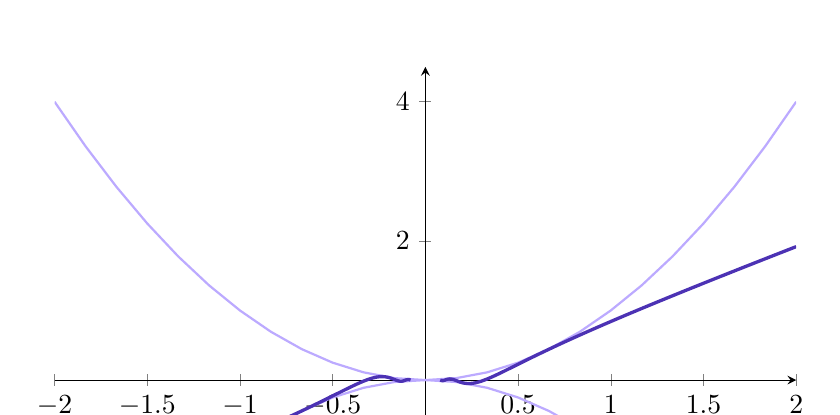
\begin{tikzpicture}\begin{axis}[width=11cm,height=6cm,axis lines=middle,xmin=-2,xmax=2,ymin=-.5,ymax=4.5]
\addplot[novelPurpleLine,thick,domain=-2:2]{x^2};\addplot[novelPurpleLine,thick,domain=-2:2]{-x^2};
\addplot[novelPurpleDark,very thick,domain=-2:-.08,samples=400]{x^2*sin(deg(1/x))};
\addplot[novelPurpleDark,very thick,domain=.08:2,samples=400]{x^2*sin(deg(1/x))};
\end{axis}\end{tikzpicture}\end{center}

\newpage
\subsection*{Studio 1.9 --- Translate Without Changing the Mathematics}
\method{A graph shows approach height, a table shows numerical stabilization, a formula supports exact simplification, and a verbal statement identifies the behavior. Check that all representations agree on direction, target input, target output, and function value.}
\quickcheck{Example 1.}{A hole at $(3,6)$ corresponds to a table approaching 6 and a simplified formula whose value would be 6.}
\quickcheck{Example 2.}{A jump graph corresponds to left and right table columns approaching different outputs.}
\quickcheck{Example 3.}{$\frac{|x-4|}{x-4}$ is $-1$ left of 4 and 1 right of 4, matching a jump graph.}
\quickcheck{Example 4.}{$\frac{x^2-9}{x-3}=x+3$ for $x\ne3$, so its graph is the line $y=x+3$ with a hole at $(3,6)$.}
\quickcheck{Example 5.}{A statement “outputs grow without bound from both sides of 2” translates to $\lim_{x\to2}f(x)=+\infty$ and a vertical asymptote $x=2$.}
\begin{skillbox}{Representation Audit}Ask four questions: What input is approached? From which side? What output is approached? What, if anything, is the actual function value?\end{skillbox}

\newpage
\subsection*{Studio 1.10 --- Discontinuity Types Have Different Causes}
\method{A removable discontinuity has a finite two-sided limit but a missing or mismatched value. A jump has unequal finite one-sided limits. An infinite discontinuity has unbounded one-sided behavior. Oscillation is also nonremovable because no single approached output exists.}
\quickcheck{Example 1.}{$\frac{x^2-1}{x-1}$ has a removable discontinuity at $x=1$.}
\quickcheck{Example 2.}{$\frac1{x-3}$ has an infinite discontinuity at $x=3$.}
\quickcheck{Example 3.}{$\frac{|x|}{x}$ has a jump discontinuity at $x=0$.}
\quickcheck{Example 4.}{$\sin(1/x)$ oscillates near 0 and has no limit there.}
\quickcheck{Example 5.}{$\tan x$ has infinite discontinuities at $x=\frac\pi2+k\pi$.}
\begin{center}\begin{tikzpicture}[scale=.8]
\draw[->] (-.2,0)--(4.3,0);\draw[->](2,-2)--(2,2.4);\draw[novelPurpleDark,thick] plot[smooth] coordinates{(.2,-1)(1,0)(1.9,.9)};\draw[novelPurpleDark,thick] plot[smooth] coordinates{(2.1,.9)(3,1.5)(4,2)};\draw[fill=white,novelPurpleDark,thick](2,.95)circle(3pt);\node at (2,-2.35){removable};
\begin{scope}[xshift=6cm]\draw[->](-.2,0)--(4.3,0);\draw[->](2,-2)--(2,2.4);\draw[novelPurpleDark,thick](.3,-1)--(1.95,-.2);\draw[novelPurpleDark,thick](2.05,1.3)--(4,2);\draw[fill=white,novelPurpleDark](2,-.2)circle(3pt);\draw[fill=white,novelPurpleDark](2,1.3)circle(3pt);\node at (2,-2.35){jump};\end{scope}
\end{tikzpicture}\end{center}

\newpage
\subsection*{Studio 1.11 --- Continuity at a Point Is a Three-Part Test}
\method{Check in order: (1) $f(c)$ is defined; (2) the two-sided limit exists; (3) the limit equals the function value. A failure at any step proves discontinuity, but name the first failed condition clearly.}
\quickcheck{Example 1.}{$f(x)=x^2+1$ is continuous at 2 because both the limit and value equal 5.}
\quickcheck{Example 2.}{A hole at $(1,4)$ with no filled point fails condition 1.}
\quickcheck{Example 3.}{A jump at $x=3$ fails condition 2, even if $f(3)$ is defined.}
\quickcheck{Example 4.}{If the limit is 6 but $f(c)=9$, condition 3 fails.}
\quickcheck{Example 5.}{For $f(x)=\begin{cases}x+2&x<1\\kx&x\ge1\end{cases}$, continuity at 1 requires $3=k$.}
\begin{skillbox}{Complete Sentence}$f$ is continuous at $c$ because $f(c)$ exists, $\lim_{x\to c}f(x)$ exists, and both quantities equal the same number.\end{skillbox}

\newpage
\subsection*{Studio 1.12 --- Continuity on Intervals Includes Domain Logic}
\method{Elementary functions are continuous on their domains. Find restrictions first: denominators cannot be zero, even-root radicands must be nonnegative, and logarithm arguments must be positive. On $[a,b]$, require right-continuity at $a$, left-continuity at $b$, and continuity inside.}
\quickcheck{Example 1.}{$\frac{x+1}{x-4}$ is continuous on $(-\infty,4)\cup(4,\infty)$.}
\quickcheck{Example 2.}{$\sqrt{2x-6}$ is continuous on $[3,\infty)$.}
\quickcheck{Example 3.}{$\ln(5-x)$ is continuous on $(-\infty,5)$.}
\quickcheck{Example 4.}{$\frac{\sqrt{x+2}}{x-1}$ is continuous on $[-2,1)\cup(1,\infty)$.}
\quickcheck{Example 5.}{$\sqrt{4-x^2}$ is continuous on $[-2,2]$, using one-sided continuity at the endpoints.}
\begin{notebox}{Endpoint Precision}At the left endpoint, compare $\lim_{x\to a^+}f(x)$ with $f(a)$. At the right endpoint, compare $\lim_{x\to b^-}f(x)$ with $f(b)$.\end{notebox}

\newpage
\subsection*{Studio 1.13 --- Repairing a Hole Means Matching the Limit}
\method{Factor or simplify the rule for $x\ne c$, evaluate the resulting limit $L$, and define $f(c)=L$. This repairs only removable discontinuities; no single assigned value can repair a jump, asymptote, or oscillation.}
\quickcheck{Example 1.}{$\frac{x^2-9}{x-3}$ is repaired at 3 by defining $f(3)=6$.}
\quickcheck{Example 2.}{$\frac{x^2+x-2}{x-1}$ is repaired at 1 by defining $f(1)=3$.}
\quickcheck{Example 3.}{$\frac{\sqrt{x+5}-3}{x-4}$ is repaired at 4 by defining the value as $1/6$.}
\quickcheck{Example 4.}{If $f(x)=\frac{x^2-4x-12}{x-6}$ for $x\ne6$, continuity requires $f(6)=8$.}
\quickcheck{Example 5.}{No value assigned at $x=0$ repairs $|x|/x$, because the two-sided limit does not exist.}
\begin{skillbox}{Geometric Meaning}Repairing a removable discontinuity fills exactly one hole at the approached height. It does not alter the surrounding curve.\end{skillbox}

\newpage
\subsection*{Studio 1.14 --- Infinite Limits Require One-Sided Sign Analysis}
\method{After locating a noncanceled denominator zero, factor the expression and make a sign chart on each side. A vertical asymptote may have $+\infty$ on both sides, $-\infty$ on both sides, or opposite signs.}
\quickcheck{Example 1.}{$\lim_{x\to2^-}\frac1{x-2}=-\infty$ and $\lim_{x\to2^+}\frac1{x-2}=+\infty$.}
\quickcheck{Example 2.}{$\lim_{x\to2}\frac1{(x-2)^2}=+\infty$.}
\quickcheck{Example 3.}{$\frac{x+1}{(x-3)(x+2)}$ has vertical asymptotes at $x=3,-2$.}
\quickcheck{Example 4.}{$\frac{x-1}{(x-1)(x+4)}$ has a hole at 1 and a vertical asymptote at $-4$.}
\quickcheck{Example 5.}{$\ln x\to-\infty$ as $x\to0^+$, so $x=0$ is a one-sided vertical asymptote.}
\begin{center}\begin{tikzpicture}\begin{axis}[width=11cm,height=6cm,axis lines=middle,xmin=-3,xmax=3,ymin=-6,ymax=6,restrict y to domain=-6:6]
\addplot[novelPurpleDark,very thick,domain=-3:-.08]{1/x};\addplot[novelPurpleDark,very thick,domain=.08:3]{1/x};\addplot[dashed,novelPurpleLine] coordinates{(0,-6)(0,6)};
\node[anchor=west] at (axis cs:.15,5){$+\infty$};\node[anchor=east] at (axis cs:-.15,-5){$-\infty$};
\end{axis}\end{tikzpicture}\end{center}

\newpage
\subsection*{Studio 1.15 --- End Behavior Depends on Dominant Growth}
\method{For rational functions, divide numerator and denominator by the highest power in the denominator or compare degrees. Lower numerator degree gives 0; equal degrees give the ratio of leading coefficients; higher numerator degree gives no horizontal asymptote and requires further end-behavior analysis.}
\quickcheck{Example 1.}{$\lim_{x\to\infty}\frac{3x+1}{x^2+4}=0$.}
\quickcheck{Example 2.}{$\lim_{x\to-\infty}\frac{5x^2-x}{2x^2+7}=\frac52$.}
\quickcheck{Example 3.}{$\lim_{x\to\infty}\frac{x^3}{x^2+1}=+\infty$; there is no horizontal asymptote.}
\quickcheck{Example 4.}{$\lim_{x\to-\infty}\frac{2x}{\sqrt{x^2+1}}=-2$ because $\sqrt{x^2}=|x|=-x$ for negative $x$.}
\quickcheck{Example 5.}{$\lim_{x\to\infty}e^{-x}=0$, while $\lim_{x\to-\infty}e^{-x}=+\infty$; the two ends need not match.}
\begin{skillbox}{Graph Interpretation}A horizontal asymptote describes what happens far left or far right. A graph may cross a horizontal asymptote; it is not a boundary.\end{skillbox}

\newpage
\subsection*{Studio 1.16 --- IVT Proves Existence, Not Location}
\method{State continuity on $[a,b]$, compute or cite the endpoint outputs, show the target $N$ lies between them, and conclude that at least one $c\in(a,b)$ satisfies $f(c)=N$. Do not claim uniqueness unless another theorem supports it.}
\quickcheck{Example 1.}{$f(x)=x^3-2$ has a zero in $(1,2)$ because $f(1)=-1$ and $f(2)=6$.}
\quickcheck{Example 2.}{$g(x)=\cos x-x$ has a zero in $(0,1)$ because $g(0)=1$ and $g(1)<0$.}
\quickcheck{Example 3.}{If continuous $h$ has $h(2)=7$ and $h(5)=-1$, then every target from $-1$ to 7 occurs at least once.}
\quickcheck{Example 4.}{Endpoint values 3 and 8 do not guarantee the target 10, though the graph could still reach it.}
\quickcheck{Example 5.}{Values with signs $+,-,+,-$ across consecutive table intervals guarantee at least three distinct zeros, one in each sign-change interval.}
\begin{center}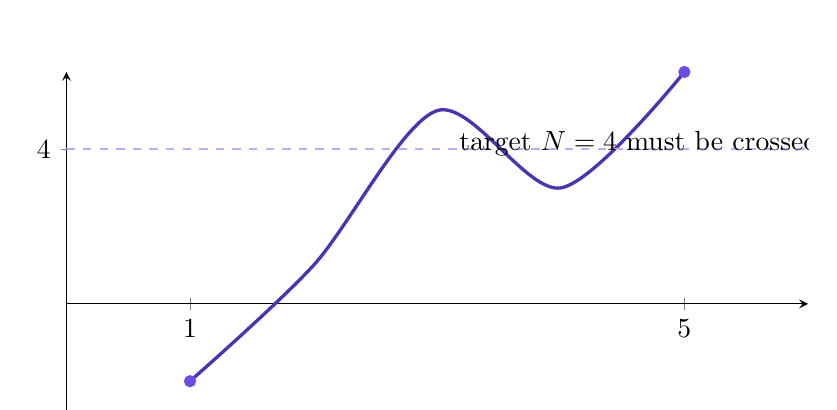
\begin{tikzpicture}\begin{axis}[width=11cm,height=6cm,axis lines=middle,xmin=0,xmax=6,ymin=-3,ymax=6,xtick={1,5},ytick={0,4}]
\addplot[novelPurpleDark,very thick,smooth] coordinates{(1,-2)(2,1)(3,5)(4,3)(5,6)};
\addplot[dashed,novelPurpleLine,thick] coordinates{(0,4)(6,4)};
\addplot[only marks,mark=*,novelPurple] coordinates{(1,-2)(5,6)};
\node[anchor=west] at (axis cs:3.1,4.15){target $N=4$ must be crossed};
\end{axis}\end{tikzpicture}\end{center}

\begin{skillbox}{Deep-Dive Completion Check}
Across the 16 studios, you should now be able to explain not only how to compute a limit, but why the chosen representation and method justify the conclusion. Rework any example whose method you cannot name before calculating.
\end{skillbox}
 \newpage
\section*{Unit 1 Synthesis}
\addcontentsline{toc}{section}{Unit 1 Synthesis}

\begin{theorybox}{Unit 1 Summary of Core Definitions}
\textbf{Limit:}
\[
\lim_{x\to c}f(x)=L
\]
means $f(x)$ approaches $L$ as $x$ approaches $c$.

\textbf{Continuity at a point:}
\begin{enumerate}
    \item $f(c)$ exists
    \item $\lim\limits_{x\to c}f(x)$ exists
    \item $\lim\limits_{x\to c}f(x)=f(c)$
\end{enumerate}

\textbf{Vertical asymptote:}
\[
x=c
\]
when the function grows without bound near $x=c$.

\textbf{Horizontal asymptote:}
\[
y=L
\]
when $f(x)\to L$ as $x\to \pm\infty$.

\textbf{Intermediate Value Theorem:} if $f$ is continuous on $[a,b]$ and $N$ lies between $f(a)$ and $f(b)$, then some $c\in(a,b)$ satisfies $f(c)=N$.
\end{theorybox}

\begin{skillbox}{What Students Should Be Able To Do by the End of Unit 1}
\begin{itemize}
    \item interpret limits verbally, graphically, numerically, and algebraically
    \item distinguish between a limit value and a function value
    \item estimate limits from graphs and tables
    \item evaluate limits by direct substitution when allowed
    \item use factoring, conjugates, and common denominators for indeterminate forms
    \item choose the most efficient procedure for a given limit
    \item apply the Squeeze Theorem in classic AP situations
    \item classify removable, jump, and infinite discontinuities
    \item test continuity at a point and over an interval
    \item identify vertical and horizontal asymptotes
    \item write a complete Intermediate Value Theorem justification
\end{itemize}
\end{skillbox}

\begin{notebox}{Most Important Unit 1 Habits}
\begin{enumerate}
    \item Do not confuse \emph{approaches} with \emph{equals}.
    \item Always test direct substitution first.
    \item If you get $\frac00$, simplify algebraically.
    \item For a two-sided limit, compare the left and right sides.
    \item A hole does not prevent the limit from existing.
    \item A vertical asymptote comes from unbounded behavior, not just from making a denominator zero before simplification.
\end{enumerate}
\end{notebox}

%
%
%
\newpage
\section*{Guided Practice Set}
\addcontentsline{toc}{section}{Guided Practice Set}

\example{Estimate graphically.}

Suppose a graph approaches $4$ from both sides as $x\to -1$, but the filled point is at $(-1,7)$. State:
\[
\lim_{x\to -1}f(x)
\qquad\text{and}\qquad
f(-1).
\]

\bigskip

\solution

\[
\lim_{x\to -1}f(x)=4
\qquad\text{and}\qquad
f(-1)=7.
\]

\bigskip

\example{Direct substitution.}

Find:
\[
\lim_{x\to 3}(2x^2-5x+1).
\]

\bigskip

\solution

\[
2(3)^2-5(3)+1=18-15+1=4.
\]

\[
\boxed{4}
\]

\bigskip

\example{Factoring.}

Find:
\[
\lim_{x\to 5}\frac{x^2-25}{x-5}.
\]

\bigskip

\solution

\[
x^2-25=(x-5)(x+5).
\]
So
\[
\frac{x^2-25}{x-5}=x+5,\qquad x\neq 5.
\]
Therefore,
\[
\lim_{x\to 5}(x+5)=10.
\]

\[
\boxed{10}
\]

\bigskip

\example{One-sided limits.}

Find
\[
\lim_{x\to 0^-}\frac{|x|}{x}
\qquad\text{and}\qquad
\lim_{x\to 0^+}\frac{|x|}{x}.
\]

\bigskip

\solution

If $x<0$, then $|x|=-x$, so
\[
\frac{|x|}{x}=\frac{-x}{x}=-1.
\]
Thus
\[
\lim_{x\to 0^-}\frac{|x|}{x}=-1.
\]

If $x>0$, then $|x|=x$, so
\[
\frac{|x|}{x}=1.
\]
Thus
\[
\lim_{x\to 0^+}\frac{|x|}{x}=1.
\]

\bigskip

\example{Continuity.}

Is
\[
f(x)=\frac{x+1}{x^2+4}
\]
continuous at $x=2$?

\bigskip

\solution

This is a rational function with denominator
\[
2^2+4=8\neq 0,
\]
so it is continuous at $x=2$.

\[
\boxed{\text{Yes}}
\]

\newpage

%
%
%
\section*{Homework / Class Exercises}
\addcontentsline{toc}{section}{Homework / Class Exercises}

\subsection*{Part A --- Core Practice}

\begin{enumerate}
    \item State in words what
    \[
    \lim_{x\to 4}f(x)=7
    \]
    means.

    \item Use direct substitution to evaluate:
    \[
    \lim_{x\to -2}(x^3+4x^2-1).
    \]

    \item Estimate from the expression by simplification:
    \[
    \lim_{x\to 2}\frac{x^2-4}{x-2}.
    \]

    \item Evaluate:
    \[
    \lim_{x\to 0}\frac{\sqrt{x+4}-2}{x}.
    \]

    \item Show that
    \[
    \lim_{x\to 0}\frac{|x|}{x}
    \]
    does not exist.

    \item Find a value of $k$ that makes the function continuous at $x=1$:
    \[
    f(x)=
    \begin{cases}
    \dfrac{x^2-1}{x-1}, & x\neq 1,\\[0.6em]
    k, & x=1.
    \end{cases}
    \]

    \item Determine whether the discontinuity of
    \[
    f(x)=\frac{x^2-1}{x-1}
    \]
    at $x=1$ is removable, jump, or infinite.

    \item Determine the vertical asymptote(s) of
    \[
    g(x)=\frac{x+3}{x^2-x-6}.
    \]

    \item Find the horizontal asymptote of
    \[
    h(x)=\frac{5x^2-3x+2}{2x^2+1}.
    \]

    \item Evaluate:
    \[
    \lim_{x\to 0}\frac{\sin 7x}{x}.
    \]
\end{enumerate}

\subsection*{Part B --- AP Style Mixed Reasoning}

\begin{enumerate}[start=11]
    \item A function $f$ satisfies:
    \[
    \lim_{x\to 3^-}f(x)=5,
    \qquad
    \lim_{x\to 3^+}f(x)=5,
    \qquad
    f(3)=-2.
    \]
    Does $\lim\limits_{x\to 3}f(x)$ exist? Is $f$ continuous at $x=3$?

    \item Find:
    \[
    \lim_{x\to \infty}\frac{3x^3+1}{x^2-4}.
    \]
    Explain whether there is a horizontal asymptote.

    \item Use the Squeeze Theorem to evaluate:
    \[
    \lim_{x\to 0}x\cos\left(\frac{1}{x}\right).
    \]

    \item For
    \[
    f(x)=
    \begin{cases}
    x+2, & x<1,\\
    4, & x=1,\\
    3x-1, & x>1,
    \end{cases}
    \]
    determine whether $f$ is continuous at $x=1$.

    \item Explain the difference between:
    \[
    \lim_{x\to c}f(x)
    \qquad\text{and}\qquad
    f(c).
    \]
\end{enumerate}

\newpage

%
%
%
\section*{Answer Key / Instructor Notes}
\addcontentsline{toc}{section}{Answer Key / Instructor Notes}

\textbf{1.} It means the outputs of $f(x)$ get arbitrarily close to $7$ as $x$ gets arbitrarily close to $4$.

\bigskip

\textbf{2.}
\[
(-2)^3+4(-2)^2-1=-8+16-1=7.
\]
\[
\boxed{7}
\]

\bigskip

\textbf{3.}
\[
\frac{x^2-4}{x-2}=\frac{(x-2)(x+2)}{x-2}=x+2.
\]
So the limit is
\[
4.
\]

\[
\boxed{4}
\]

\bigskip

\textbf{4.}
Rationalize:
\[
\frac{\sqrt{x+4}-2}{x}\cdot \frac{\sqrt{x+4}+2}{\sqrt{x+4}+2}
=
\frac{x+4-4}{x(\sqrt{x+4}+2)}
=
\frac{1}{\sqrt{x+4}+2}.
\]
Now let $x\to 0$:
\[
\frac{1}{2+2}=\frac14.
\]

\[
\boxed{\frac14}
\]

\bigskip

\textbf{5.}
\[
\lim_{x\to 0^-}\frac{|x|}{x}=-1,
\qquad
\lim_{x\to 0^+}\frac{|x|}{x}=1.
\]
Since they are different, the two-sided limit does not exist.

\bigskip

\textbf{6.}
\[
\frac{x^2-1}{x-1}=\frac{(x-1)(x+1)}{x-1}=x+1.
\]
So
\[
k=\lim_{x\to 1}(x+1)=2.
\]

\[
\boxed{k=2}
\]

\bigskip

\textbf{7.}
The factor cancels and leaves a hole, so the discontinuity is \textbf{removable}.

\bigskip

\textbf{8.}
\[
x^2-x-6=(x-3)(x+2).
\]
Thus the vertical asymptotes occur at
\[
x=3,\qquad x=-2.
\]

\[
\boxed{x=3,\,-2}
\]

\bigskip

\textbf{9.}
Degrees are equal, so the horizontal asymptote is the ratio of leading coefficients:
\[
y=\frac52.
\]

\[
\boxed{y=\frac52}
\]

\bigskip

\textbf{10.}
\[
\frac{\sin 7x}{x}
=
7\cdot\frac{\sin 7x}{7x}\to 7.
\]

\[
\boxed{7}
\]

\bigskip

\textbf{11.}
Yes,
\[
\lim_{x\to 3}f(x)=5
\]
exists because the two one-sided limits agree. But $f(3)=-2$, so the function is \textbf{not continuous} at $x=3$.

\bigskip

\textbf{12.}
The degree of the numerator is greater than the degree of the denominator, so the function grows without bound in magnitude. There is \textbf{no horizontal asymptote}. The limit is not finite.

\bigskip

\textbf{13.}
Since
\[
-1\le \cos\left(\frac1x\right)\le 1,
\]
multiplying by $x$ and squeezing carefully leads to
\[
-x\le x\cos\left(\frac1x\right)\le x
\quad\text{if }x>0,
\]
and similarly the bound still forces the expression to $0$ from both sides. Thus:
\[
\boxed{0}
\]

\bigskip

\textbf{14.}
Left-hand limit:
\[
\lim_{x\to 1^-}f(x)=1+2=3.
\]
Right-hand limit:
\[
\lim_{x\to 1^+}f(x)=3(1)-1=2.
\]
Since these are not equal, the limit does not exist, so the function is \textbf{not continuous} at $x=1$.

\bigskip

\textbf{15.}
$\lim_{x\to c}f(x)$ describes the value the function approaches near $x=c$, while $f(c)$ is the actual defined output at $x=c$. They may be equal, but they do not have to be.

%
%
%
\newpage
\section*{Unit 1 Final Teaching Checklist}
\addcontentsline{toc}{section}{Unit 1 Final Teaching Checklist}

\begin{skillbox}{Before Moving to Derivatives, Students Should Comfortably Handle}
\begin{itemize}
    \item interpreting limits from graphs and tables
    \item distinguishing the function value from the limiting value
    \item evaluating limits by direct substitution and by algebraic manipulation
    \item using one-sided limits
    \item classifying discontinuities
    \item checking continuity at points and on intervals
    \item recognizing vertical and horizontal asymptotes
    \item applying the Intermediate Value Theorem with all hypotheses stated
\end{itemize}
\end{skillbox}

\vfill

\begin{center}
{\Large\bfseries\color{novelPurpleDark} End of Unit 1}\\[0.5em]
{\large\color{novelPurple} Limits and Continuity}
\end{center}

\end{document}
